\documentclass[11pt,a4paper]{report}
\usepackage[top=20mm,bottom=20mm,left=22mm,right=18mm]{geometry}
\usepackage{setspace}\setstretch{1.05}
\setlength{\parskip}{2.5pt plus 0.5pt minus 0.5pt}
\setlength{\parindent}{1.3em}
\usepackage{amsmath,amssymb,amsfonts}
\usepackage{graphicx}\graphicspath{{figures/}}
\usepackage{booktabs,tabularx,multirow}
\usepackage[table]{xcolor}
\usepackage{pifont}
\newcommand{\cmark}{\ding{51}}%
\usepackage[font=small,labelfont=bf,skip=4pt]{caption}
\usepackage{enumerate}
\usepackage{hyperref}\hypersetup{colorlinks,linkcolor=blue!70!black,citecolor=blue!70!black,urlcolor=blue!70!black}
\usepackage[numbers,sort&compress]{natbib}
\setlength{\bibsep}{3pt}
\pagestyle{headings}

%% Tighten float spacing
\setlength{\floatsep}{8pt plus 2pt minus 2pt}
\setlength{\textfloatsep}{10pt plus 2pt minus 2pt}
\setlength{\intextsep}{8pt plus 2pt minus 2pt}
\setlength{\abovecaptionskip}{4pt}
\setlength{\belowcaptionskip}{3pt}

\usepackage{etoolbox}
\makeatletter
%% Continuous chapter layout with clean separation
\patchcmd{\chapter}{\clearpage}{\par\vspace{16pt}}{}{}
\def\@makechapterhead#1{%
  \vspace*{6\p@}%
  {\parindent \z@ \raggedright \normalfont
    \ifnum \c@secnumdepth >\m@ne
        \large\bfseries \@chapapp\space \thechapter\quad---\quad #1
        \par\nobreak
        \vskip 6\p@
    \fi
  }}
\def\@makeschapterhead#1{%
  \vspace*{6\p@}%
  {\parindent \z@ \raggedright
    \normalfont
    \large \bfseries #1\par\nobreak
    \vskip 6\p@
  }}
\makeatother

\newcommand{\E}{\mathbb{E}}
\newcommand{\R}{\mathbb{R}}
\DeclareMathOperator{\clip}{clip}
\DeclareMathOperator{\Dir}{Dirichlet}

\begin{document}

%% ===== TITLE PAGE (Image 1 Style) =====
\begin{titlepage}
\centering
\vspace*{0.2cm}
{\large B.Tech Project-I report submitted to\par}
\vspace{0.2cm}
{\large Indian Institute of Technology Kharagpur\par}
\vspace{0.2cm}
{\normalsize in partial fulfilment for the award of the degree of\par}
\vspace{0.2cm}
{\large\bfseries Bachelor of Technology (B. Tech)\par}
\vspace{0.15cm}
{\normalsize in\par}
\vspace{0.15cm}
{\large Industrial and Systems Engineering\par}
\vspace{0.8cm}
{\normalsize by\par}
\vspace{0.2cm}
{\large\bfseries Ritam Mondal\par}
\vspace{0.15cm}
{\normalsize\bfseries (23IM30018)\par}
\vspace{0.8cm}
{\normalsize Under the supervision of\par}
\vspace{0.2cm}
{\large\bfseries Professor Abhisek Sharma\par}
\vspace{0.8cm}

\includegraphics[width=3.2cm]{figures/iitkgp_logo.png}\par
\vspace{0.8cm}
{\large\bfseries Department of Industrial and Systems Engineering\par}
\vspace{0.2cm}
{\large Indian Institute of Technology Kharagpur\par}
\vspace{0.2cm}
{\normalsize Autumn Semester, 2026--27\par}
\vspace{0.2cm}
{\normalsize November 2026\par}
\vfill
\end{titlepage}

\pagenumbering{roman}
\setcounter{page}{1}

%% ===== DECLARATION PAGE (Image 2 Style) =====
\newpage
\thispagestyle{plain}
\begin{center}
\vspace*{1.5cm}
{\large\bfseries DECLARATION\par}
\end{center}
\vspace{1.5cm}
\noindent I certify that
\vspace{0.5cm}
\begin{enumerate}[(a)]
  \setlength{\itemsep}{14pt}
  \item The work contained in this report has been done by me under the guidance of my supervisor.
  \item The work has not been submitted to any other Institute for any degree or diploma.
  \item I have conformed to the norms and guidelines given in the Ethical Code of Conduct of the Institute.
  \item Whenever I have used materials (data, theoretical analysis, figures, and text) from other sources, I have given due credit to them by citing them in the text of the thesis and giving their details in the references. Further, I have taken permission from the copyright owners of the sources, whenever necessary.
\end{enumerate}

\vspace{4.0cm}
\noindent
\begin{minipage}[t]{0.5\textwidth}
Date: November 1, 2026\\[6pt]
Place: Kharagpur
\end{minipage}
\hfill
\begin{minipage}[t]{0.45\textwidth}
\raggedleft
(Ritam Mondal)\\[6pt]
(23IM30018)
\end{minipage}

%% ===== CERTIFICATE PAGE (Image 3 Style) =====
\newpage
\thispagestyle{plain}
\begin{center}
\vspace*{0.2cm}
{\bfseries DEPARTMENT OF INDUSTRIAL AND SYSTEMS ENGINEERING\par}
\vspace{0.15cm}
{\bfseries INDIAN INSTITUTE OF TECHNOLOGY KHARAGPUR\par}
\vspace{0.15cm}
{\bfseries KHARAGPUR -- 721302, INDIA\par}
\vspace{0.8cm}

\includegraphics[width=2.8cm]{figures/iitkgp_logo.png}\par
\vspace{0.8cm}
{\large\bfseries CERTIFICATE\par}
\end{center}
\vspace{0.8cm}
\noindent This is to certify that the project report entitled ``\textbf{Risk-Aware Deep Reinforcement Learning for Daily Portfolio Allocation}'' submitted by \textbf{Ritam Mondal} (Roll No. 23IM30018) to Indian Institute of Technology Kharagpur towards partial fulfilment of requirements for the award of degree of Bachelor of Technology in Industrial and Systems Engineering is a record of bona fide work carried out under my supervision and guidance during Autumn Semester, 2026--27.

\vspace{3.5cm}
\noindent
\begin{minipage}[t]{0.5\textwidth}
Date: November 1, 2026\\[6pt]
Place: Kharagpur
\end{minipage}
\hfill
\begin{minipage}[t]{0.48\textwidth}
\raggedleft
Professor Abhisek Sharma\\[4pt]
Department of Industrial and Systems Engineering\\[4pt]
Indian Institute of Technology Kharagpur\\[4pt]
Kharagpur -- 721302, India
\end{minipage}

%% ===== ACKNOWLEDGEMENT & ABSTRACT =====
\newpage
\thispagestyle{plain}
\chapter*{Acknowledgement and Abstract}
\addcontentsline{toc}{chapter}{Acknowledgement and Abstract}

\noindent\textbf{Acknowledgement:}\par
I express my deepest gratitude to my supervisor, Professor Abhisek Sharma, for his insightful guidance, intellectual mentorship, and continuous encouragement throughout this B.Tech.\ Project. His domain expertise in financial engineering, operations research, and sequential decision processes has been instrumental in shaping the theoretical and empirical methodology of this thesis. I also extend my gratitude to the Department of Industrial and Systems Engineering, Indian Institute of Technology Kharagpur, for providing the necessary computing resources, and to my peers and family for their unwavering support.

\vspace{0.6cm}
\noindent\textbf{Abstract:}\par
Daily portfolio allocation is difficult to automate because financial markets exhibit low signal-to-noise ratios, non-stationary dynamics, and only partial observability of the true underlying economic state. Deep reinforcement learning (DRL) research has separately proposed temporal memory, risk-aware reward shaping, and turnover regularization to address these challenges, but such mechanisms are rarely isolated under identical experimental conditions, making it difficult to attribute performance differences to any single design choice.

This report presents a rigorous, controlled four-stage ablation framework: (i)~Model M1: Proximal Policy Optimisation (PPO) with a feedforward Multi-Layer Perceptron (MLP) baseline and net return reward; (ii)~Model M2: PPO with a recurrent Long Short-Term Memory (LSTM) encoder and net return reward; (iii)~Model M3: LSTM-PPO with recursive Differential Sharpe Ratio (DSR) reward shaping; and (iv)~Model M4: LSTM-PPO with DSR reward and explicit quadratic turnover regularisation ($\lambda_{\text{turn}} = 0.1$). All models parameterise portfolio allocations over a continuous Dirichlet distribution, naturally satisfying non-negativity and budget simplex constraints with an explicit cash reserve.

Models are trained and evaluated on the same daily equity universe of ten major National Stock Exchange of India (NSE) stocks, identical thirteen causal technical indicators, realistic proportional transaction costs ($0.1\%$), and four rolling walk-forward folds across 2018--2025 over multiple random seeds. Results reveal that temporal memory (M2) substantially enhances out-of-sample Sharpe ratio ($+0.201$) while cutting daily turnover by $57\%$. Turnover regularisation (M4) effectively suppresses transaction costs to $0.97\%$ of starting capital and achieves the shallowest maximum drawdown ($-16.04\%$). However, learned risk-aversion leads the agents to hold conservative cash buffers, resulting in cash drag against a fully-invested passive Equal-Weight benchmark during an extended bull market.

\medskip\noindent\textbf{Keywords:} Deep Reinforcement Learning, Portfolio Management, Proximal Policy Optimisation, Dirichlet Policy, Differential Sharpe Ratio, Turnover Regularisation, POMDP, Walk-Forward Validation.

%% ===== TABLE OF CONTENTS =====
\newpage
\thispagestyle{plain}
\begin{singlespace}
\setcounter{tocdepth}{1}
\tableofcontents
\end{singlespace}

\newpage
\pagenumbering{arabic}
\setcounter{page}{1}

%% ===== MAIN CHAPTERS =====
\chapter{Introduction}
\label{ch:intro}

\section{Background and Motivation}
Daily portfolio allocation requires selecting asset weights repeatedly as prices and market conditions change. These decisions must balance investment returns, financial risk, and transaction costs. A policy based only on current-day indicators may overlook recent market dynamics, while return-based rewards and frequent rebalancing may lead to risky or costly allocations. This study examines three components within a common PPO-based framework: temporal memory through an LSTM encoder, risk-aware reward shaping through the Differential Sharpe Ratio (DSR), and turnover control through a quadratic weight-change penalty. Their contributions are evaluated through four controlled models (M1--M4) using chronological walk-forward testing on ten NSE equities, with an Equal-Weight portfolio as the benchmark.

\chapter{Literature Review}
\label{ch:lit_review}

The application of deep reinforcement learning to algorithmic trading and portfolio management has developed rapidly across policy optimisation, sequence modeling, risk-aware rewards, and evaluation standards. This chapter presents a focused review of the core literature directly motivating our research.

\noindent\textbf{Schulman et al. (2017)} \citep{schulman2017proximal} developed Proximal Policy Optimisation (PPO), introducing a clipped surrogate objective that restricts policy update ratios within an $\epsilon$-neighbourhood around the previous policy. This provides stable gradient updates in continuous control environments without the excessive hyperparameter sensitivity of earlier policy gradient methods. While PPO provides an effective actor--critic foundation, its application to continuous multi-asset portfolio management requires adapting the action distribution to the portfolio simplex and formulating risk-sensitive rewards.

\noindent\textbf{Zou et al. (2024)} \citep{zou2024novel} proposed an equity trading architecture that combines a recurrent LSTM encoder with PPO policy optimization. Using a 30-day historical window and a 512-dimensional hidden representation, their system showed that multi-day sequential features capture price momentum more effectively than single-day snapshots. However, their policy rewards focused on nominal trading profit for individual equities rather than risk-adjusted continuous portfolio allocation across a multi-asset universe.

\noindent\textbf{Millea (2021)} \citep{millea2021deep} provided a survey of reinforcement learning in quantitative trading, emphasizing the need for standardised evaluation protocols and risk-sensitive objective functions. The author reviewed the Differential Sharpe Ratio (DSR), which updates running first and second return moments recursively to reward risk-adjusted returns online. While DSR provides an analytical alternative to raw returns, its empirical interaction with recurrent encoders and execution frictions under standard actor--critic methods warrants systematic evaluation.

\noindent\textbf{Liu et al. (2024)} \citep{liu2024dynamic} introduced the FinRL-Meta framework, establishing dynamic market environments and a rolling walk-forward evaluation protocol. Their rolling train--validation--test scheme advances windows chronologically across market cycles, directly mitigating look-ahead bias and macroeconomic regime shifts. Although their work established rigorous financial testing standards, their continuous portfolio experiments evaluated fixed configurations without isolating the separate impacts of sequence encoders or turnover penalties.

\noindent\textbf{Wang and Liu (2025)} \citep{wang2025risk} developed a risk-sensitive reinforcement learning framework for portfolio allocation across volatile market regimes, incorporating downside risk penalties and turnover control into policy learning. Their results confirmed that penalising volatility and trading frictions preserves capital during market downturns. However, because their experiments modified the sequence backbone, reward function, and trading constraints simultaneously, the individual contribution of each mechanism was not isolated.

\noindent\textbf{Yang et al. (2022)} \citep{yang2022selective} introduced a continuous portfolio allocation algorithm parameterised over a multivariate Dirichlet distribution. Unlike heuristic Gaussian clipping or post-hoc Softmax normalization, sampling actions from a Dirichlet distribution inherently constrains target portfolio allocations to the unit simplex manifold. While their study demonstrated the mathematical appeal of Dirichlet policies in off-policy trading, it did not investigate recurrent temporal representations or explicit transaction-cost regularization.

\chapter{Research Gap and Problem Formulation}
\label{ch:gap}

\section{Identified Research Gap}
While significant progress has been made across temporal modeling, risk-sensitive rewards, and walk-forward validation protocols, existing studies have typically evaluated these mechanisms within isolated frameworks using divergent market universes, varied cost assumptions, and concurrent architectural changes. 

Based on the literature reviewed, there remains a clear need for controlled empirical comparisons that systematically isolate the contributions of temporal memory, risk-aware rewards, and turnover regularization under a common, realistic experimental setup. Without holding the asset universe, feature set, transaction-cost model, training budget, and chronological evaluation protocol constant, it is difficult to determine whether reported differences in out-of-sample performance stem from the sequence encoder, the reward function, turnover control, or differences in the experimental setup itself.

Table~\ref{tab:positioning} positions this thesis relative to the reviewed literature, highlighting the controlled single-factor ablation design adopted here.

\begin{table}[htbp]
\centering
\scriptsize
\setlength{\tabcolsep}{3.5pt}
\caption{Positioning of this work relative to the reviewed literature.}
\label{tab:positioning}
\begin{tabularx}{\textwidth}{>{\raggedright\arraybackslash}p{2.8cm}>{\centering\arraybackslash}X>{\centering\arraybackslash}p{3.1cm}>{\centering\arraybackslash}p{2.4cm}>{\centering\arraybackslash}p{2.5cm}>{\centering\arraybackslash}X}
\toprule
\textbf{Paper} & \textbf{Temporal Memory} & \textbf{Risk-Aware / Reward} & \textbf{Turnover Control} & \textbf{Continuous Allocation} & \textbf{Controlled Ablation} \\
\midrule
Millea (2021) \citep{millea2021deep} & & \cmark~\textit{(risk-aware rewards discussed)} & & & \\
Zou et al. (2024) \citep{zou2024novel} & \cmark & & & & \\
Huang et al. (2024) \citep{huang2024self} & & \cmark & & & \\
Liu et al. (2024) \citep{liu2024dynamic} & & & & \cmark~\textit{(portfolio weights)} & \\
Wang \& Liu (2025) \citep{wang2025risk} & & \cmark~\textit{(risk-sensitive reward)} & \cmark & \cmark & \\
Yang et al. (2022) \citep{yang2022selective} & & & & \cmark~\textit{(Dirichlet distribution)} & \\
\midrule
\textbf{This work} & \cmark & \cmark~\textit{(DSR)} & \cmark~\textit{(turnover penalty)} & \cmark & \cmark \\
\bottomrule
\end{tabularx}
\end{table}

\section{POMDP Formulation of Daily Portfolio Allocation}
\label{sec:pomdp_formulation}
We formulate daily portfolio allocation as a Partially Observable Markov Decision Process (POMDP), defined by the 7-tuple:
\begin{equation}
\mathcal{P} = \langle \mathcal{S}, \mathcal{A}, \mathcal{T}, \mathcal{R}, \Omega, \mathcal{O}, \gamma \rangle,
\end{equation}
where $\mathcal{S}$ is the unobservable state space, $\mathcal{A}$ is the action space, $\mathcal{T}$ represents transition dynamics, $\mathcal{R}$ is the reward function, $\Omega$ is the observation space, $\mathcal{O}$ is the observation probability distribution, and $\gamma \in [0, 1)$ is the discount factor.

\subsection{Why Daily Financial Trading is a POMDP}
In a fully observable Markov Decision Process (MDP), the Markov property requires that future state transitions depend solely on the current state and action: $\mathbb{P}(\mathbf{s}_{t+1} \mid \mathbf{s}_t, \mathbf{a}_t) = \mathbb{P}(\mathbf{s}_{t+1} \mid \mathbf{s}_t, \dots, \mathbf{s}_0)$. In financial trading, this assumption does not hold when applied directly to observable market indicators:
\begin{enumerate}
    \item \textbf{Unobservable True Market State $\mathcal{S}$:} The complete economic state of financial markets includes macroeconomic fundamentals, central bank expectations, institutional limit order book queues, private liquidity flows, and participant psychology. These variables are latent and cannot be directly observed by an agent trading from public daily price feeds.
    \item \textbf{Partial and Noisy Observations $\Omega$:} The agent receives only an observation vector $\mathbf{o}_t \in \Omega$ drawn from the observation model $\mathcal{O}(\mathbf{o}_t \mid \mathbf{s}_t)$, consisting of daily open, high, low, close prices, trading volumes, and derived technical indicators.
    \item \textbf{Non-Markovian Indicator Dynamics:} An identical single-day technical observation vector (e.g., RSI = 65, MACD crossover) can result in completely different future price movements depending on latent market conditions (such as the beginning of a sustained trend versus an institutional distribution phase).
\end{enumerate}
Because single-day observations $\mathbf{o}_t$ do not satisfy the Markov property, an agent benefits from maintaining an internal temporal representation or belief state $b(\mathbf{s}_t)$ over historical observation sequences $\mathbf{F}_t = [\mathbf{s}_{t-W+1}, \dots, \mathbf{s}_t]$. In this work, recurrent neural networks (LSTM) are used to construct this temporal summary $\mathbf{h}_t \approx b(\mathbf{s}_t)$ end-to-end, directly mitigating the effects of partial observability.

\subsection{Action Space $\mathcal{A}$ and Simplex Manifold}
The portfolio consists of $N = 10$ risky equities and $1$ cash account, yielding an action dimension of $M = N + 1 = 11$. The action vector $\mathbf{a}_t = [a_{t,1}, \dots, a_{t,N+1}]^\top$ represents target portfolio weights, strictly constrained to lie on the unit simplex:
\begin{equation}
\label{eq:simplex_constraint}
\mathcal{A} \equiv \Delta^N = \left\{ \mathbf{w}_t \in \mathbb{R}^{N+1} \;\middle|\; w_{i,t} \ge 0 \; \forall i, \quad \sum_{i=1}^{N} w_{i,t} + w_{\text{cash},t} = 1 \right\}.
\end{equation}
Following \citet{yang2022selective}, this constraint is enforced directly by parameterising the actor network over a multivariate Dirichlet distribution, eliminating the need for heuristic projection or unconstrained Gaussian clipping.

\chapter{Dataset and Experimental Methodology}
\label{ch:data}

\section{Equity Universe and Data Acquisition}
The experimental stock universe comprises $N = 10$ prominent large-cap equities actively traded on the National Stock Exchange of India (NSE), spanning diverse economic sectors:
\begin{enumerate}
    \setlength{\itemsep}{1pt}
    \item \textbf{RELIANCE.NS} (Energy and Petrochemicals / Conglomerate)
    \item \textbf{TCS.NS} (Information Technology Services)
    \item \textbf{HDFCBANK.NS} (Private Commercial Banking)
    \item \textbf{ICICIBANK.NS} (Private Commercial Banking)
    \item \textbf{ITC.NS} (Consumer Goods and Diversified Conglomerate)
    \item \textbf{HINDUNILVR.NS} (Fast-Moving Consumer Goods)
    \item \textbf{LT.NS} (Engineering and Infrastructure Construction)
    \item \textbf{SUNPHARMA.NS} (Pharmaceuticals and Healthcare)
    \item \textbf{MARUTI.NS} (Automotive Manufacturing)
    \item \textbf{BHARTIARTL.NS} (Telecommunications and Digital Services)
\end{enumerate}
In addition to these ten equities, the portfolio includes an explicit cash asset (Asset 11), providing the agent with the operational flexibility to hold liquidity and de-risk during volatile market phases.

Daily price and volume records were acquired from Yahoo Finance via the \texttt{yfinance} API spanning 1 January 2009 to 31 December 2025. Data acquisition utilized \texttt{auto\_adjust=True}: price series (Open, High, Low, and Close) are backward-adjusted for both stock splits and cash dividends, whereas trading volume is adjusted for splits. Data from 2009--2010 serves as an initial burn-in buffer to initialize 200-day moving averages, ensuring that all technical indicators are fully settled by 1 January 2011. The common trading calendar comprises 3,699 active trading days.

\section{Feature Engineering and Market Indicators}
For each asset $i \in \{1, \dots, N\}$ on trading day $t$, a compact feature vector $\mathbf{f}_{i,t} \in \mathbb{R}^{13}$ is computed using causal market and technical price transformations. To ensure cross-asset comparability, features are normalized by prevailing prices or rolling averages:

\begin{enumerate}
    \setlength{\itemsep}{2pt}
    \item \textbf{Daily Log Return ($f_{1,i,t}$):} $r_{i,t}^{\text{log}} = \ln\left( C_{i,t} / C_{i,t-1} \right)$.
    \item \textbf{Close-to-Open Relative Return ($f_{2,i,t}$):} $o_{i,t}^{\text{rel}} = C_{i,t} / O_{i,t} - 1$.
    \item \textbf{High-to-Low Relative Spread ($f_{3,i,t}$):} $hl_{i,t}^{\text{rel}} = H_{i,t} / L_{i,t} - 1$.
    \item \textbf{Normalized Relative Volume ($f_{4,i,t}$):} $v_{i,t}^{\text{rel}} = \ln\left( V_{i,t} / \text{SMA}_{20}(V_{i,t}) \right)$.
    \item \textbf{50-day EMA Relative Deviation ($f_{5,i,t}$):} $ema_{50,i,t}^{\text{rel}} = C_{i,t} / \text{EMA}_{50}(C_{i,t}) - 1$, with smoothing multiplier $\alpha_n = \frac{2}{n+1}$.
    \item \textbf{200-day EMA Relative Deviation ($f_{6,i,t}$):} $ema_{200,i,t}^{\text{rel}} = C_{i,t} / \text{EMA}_{200}(C_{i,t}) - 1$.
    \item \textbf{Relative Strength Index ($f_{7,i,t}$):} Wilder's 14-period RSI centered around zero:
    \begin{equation}
    \text{RS}_{i,t} = \frac{\bar{U}_{i,t}}{\bar{D}_{i,t} + 10^{-8}}, \quad \text{RSI}_{i,t} = 100 - \frac{100}{1 + \text{RS}_{i,t}}, \quad f_{7,i,t} = \frac{\text{RSI}_{i,t}}{100} - 0.5.
    \end{equation}
    \item \textbf{Moving Average Convergence Divergence ($f_{8,i,t}$):} Normalized trend divergence:
    \begin{equation}
    \text{MACD}_{i,t} = \frac{\text{EMA}_{12}(C_{i,t}) - \text{EMA}_{26}(C_{i,t})}{C_{i,t}}.
    \end{equation}
    \item \textbf{MACD Signal Line ($f_{9,i,t}$):} $\text{Signal}_{i,t} = \text{EMA}_9(\text{MACD}_{i,t}) / C_{i,t}$.
    \item \textbf{Average True Range ($f_{10,i,t}$):} Normalized price volatility:
    \begin{equation}
    \text{ATR}_{i,t}^{\text{rel}} = \frac{\text{SMA}_{14}(\text{TR}_{i,t})}{C_{i,t}}, \quad \text{where } \text{TR}_t = \max(H_t - L_t, |H_t - C_{t-1}|, |L_t - C_{t-1}|).
    \end{equation}
    \item \textbf{Bollinger Band \%B ($f_{11,i,t}$):} Position relative to 2-standard-deviation envelopes:
    \begin{equation}
    \%B_{i,t} = \frac{C_{i,t} - \text{LB}_{i,t}}{\text{UB}_{i,t} - \text{LB}_{i,t} + 10^{-8}}.
    \end{equation}
    \item \textbf{Bollinger Bandwidth ($f_{12,i,t}$):} Volatility width: $\text{BW}_{i,t} = (\text{UB}_{i,t} - \text{LB}_{i,t}) / \text{MB}_{i,t}$.
    \item \textbf{Average Directional Index ($f_{13,i,t}$):} Wilder's 14-period normalized trend: $\text{ADX}_{i,t}^{\text{norm}} = \text{ADX}_{14,i,t} / 100$.
\end{enumerate}

\section{State Representation and Temporal Sequences}
The instantaneous observation vector concatenates the 13 features across all $N = 10$ equities ($130$ market features) with the current portfolio weight vector $\mathbf{w}_t^{\text{cur}} \in \mathbb{R}^{N+1}$ (10 equities plus cash, 11 weights):
\begin{align}
\mathbf{x}_t &= \text{concat}\left(\mathbf{f}_{1,t}, \dots, \mathbf{f}_{N,t}\right) \in \mathbb{R}^{130}, \\
\mathbf{s}_t &= \left[ \mathbf{x}_t^\top, \; (\mathbf{w}_t^{\text{cur}})^\top \right]^\top \in \mathbb{R}^{141}.
\end{align}
The total daily state dimension is $D_{\text{state}} = 141$. For models using recurrent memory (M2--M4), a sliding historical window of $W = 30$ trading days is maintained:
\begin{equation}
\mathbf{F}_t = \left[ \mathbf{s}_{t-W+1}, \dots, \mathbf{s}_t \right]^\top \in \mathbb{R}^{30 \times 141}.
\end{equation}
Feature standardization is fitted strictly on the training partition of each fold using mean $\boldsymbol{\mu}_{\text{train}}$ and standard deviation $\boldsymbol{\sigma}_{\text{train}}$, with standardized values clipped to $[-5.0, 5.0]$. All features use causal backward operators, preventing look-ahead leakage.

\section{Walk-Forward Evaluation Protocol}
Following \citet{liu2024dynamic}, models are trained and tested using an 8-year rolling-origin walk-forward protocol across four folds. Each fold consists of 6 years of training data, 1 year of validation data, and 2 years of held-out out-of-sample test data, advancing by 2 years per fold (Table~\ref{tab:folds_overview} and Figure~\ref{fig:walk_forward}).

\begin{table}[htbp]
\centering
\small
\setlength{\tabcolsep}{4pt}
\caption{Chronological specification of the four walk-forward folds.}
\label{tab:folds_overview}
\begin{tabularx}{\textwidth}{c>{\centering\arraybackslash}X>{\centering\arraybackslash}X>{\centering\arraybackslash}Xcc}
\toprule
\textbf{Fold} & \textbf{Training Period (6y)} & \textbf{Validation Period (1y)} & \textbf{Test Period (2y)} & \textbf{Training Trading Days} & \textbf{Test Trading Days} \\
\midrule
1 & 2011-01-01 to 2016-12-31 & 2017-01-01 to 2017-12-31 & 2018-01-01 to 2019-12-31 & 1,478 & 489 \\
2 & 2013-01-01 to 2018-12-31 & 2019-01-01 to 2019-12-31 & 2020-01-01 to 2021-12-31 & 1,475 & 496 \\
3 & 2015-01-01 to 2020-12-31 & 2021-01-01 to 2021-12-31 & 2022-01-01 to 2023-12-31 & 1,476 & 495 \\
4 & 2017-01-01 to 2022-12-31 & 2023-01-01 to 2023-12-31 & 2024-01-01 to 2025-12-31 & 1,479 & 494 \\
\bottomrule
\end{tabularx}
\end{table}

The test periods are non-overlapping and span 2018 through 2025. It is important to distinguish the number of historical trading days in the dataset splits ($\approx 1,478$ training days and $\approx 490$ test days) from the reinforcement learning training budget, which is fixed at 300,000 environment interaction steps across all models.

\begin{figure}[htbp]
\centering
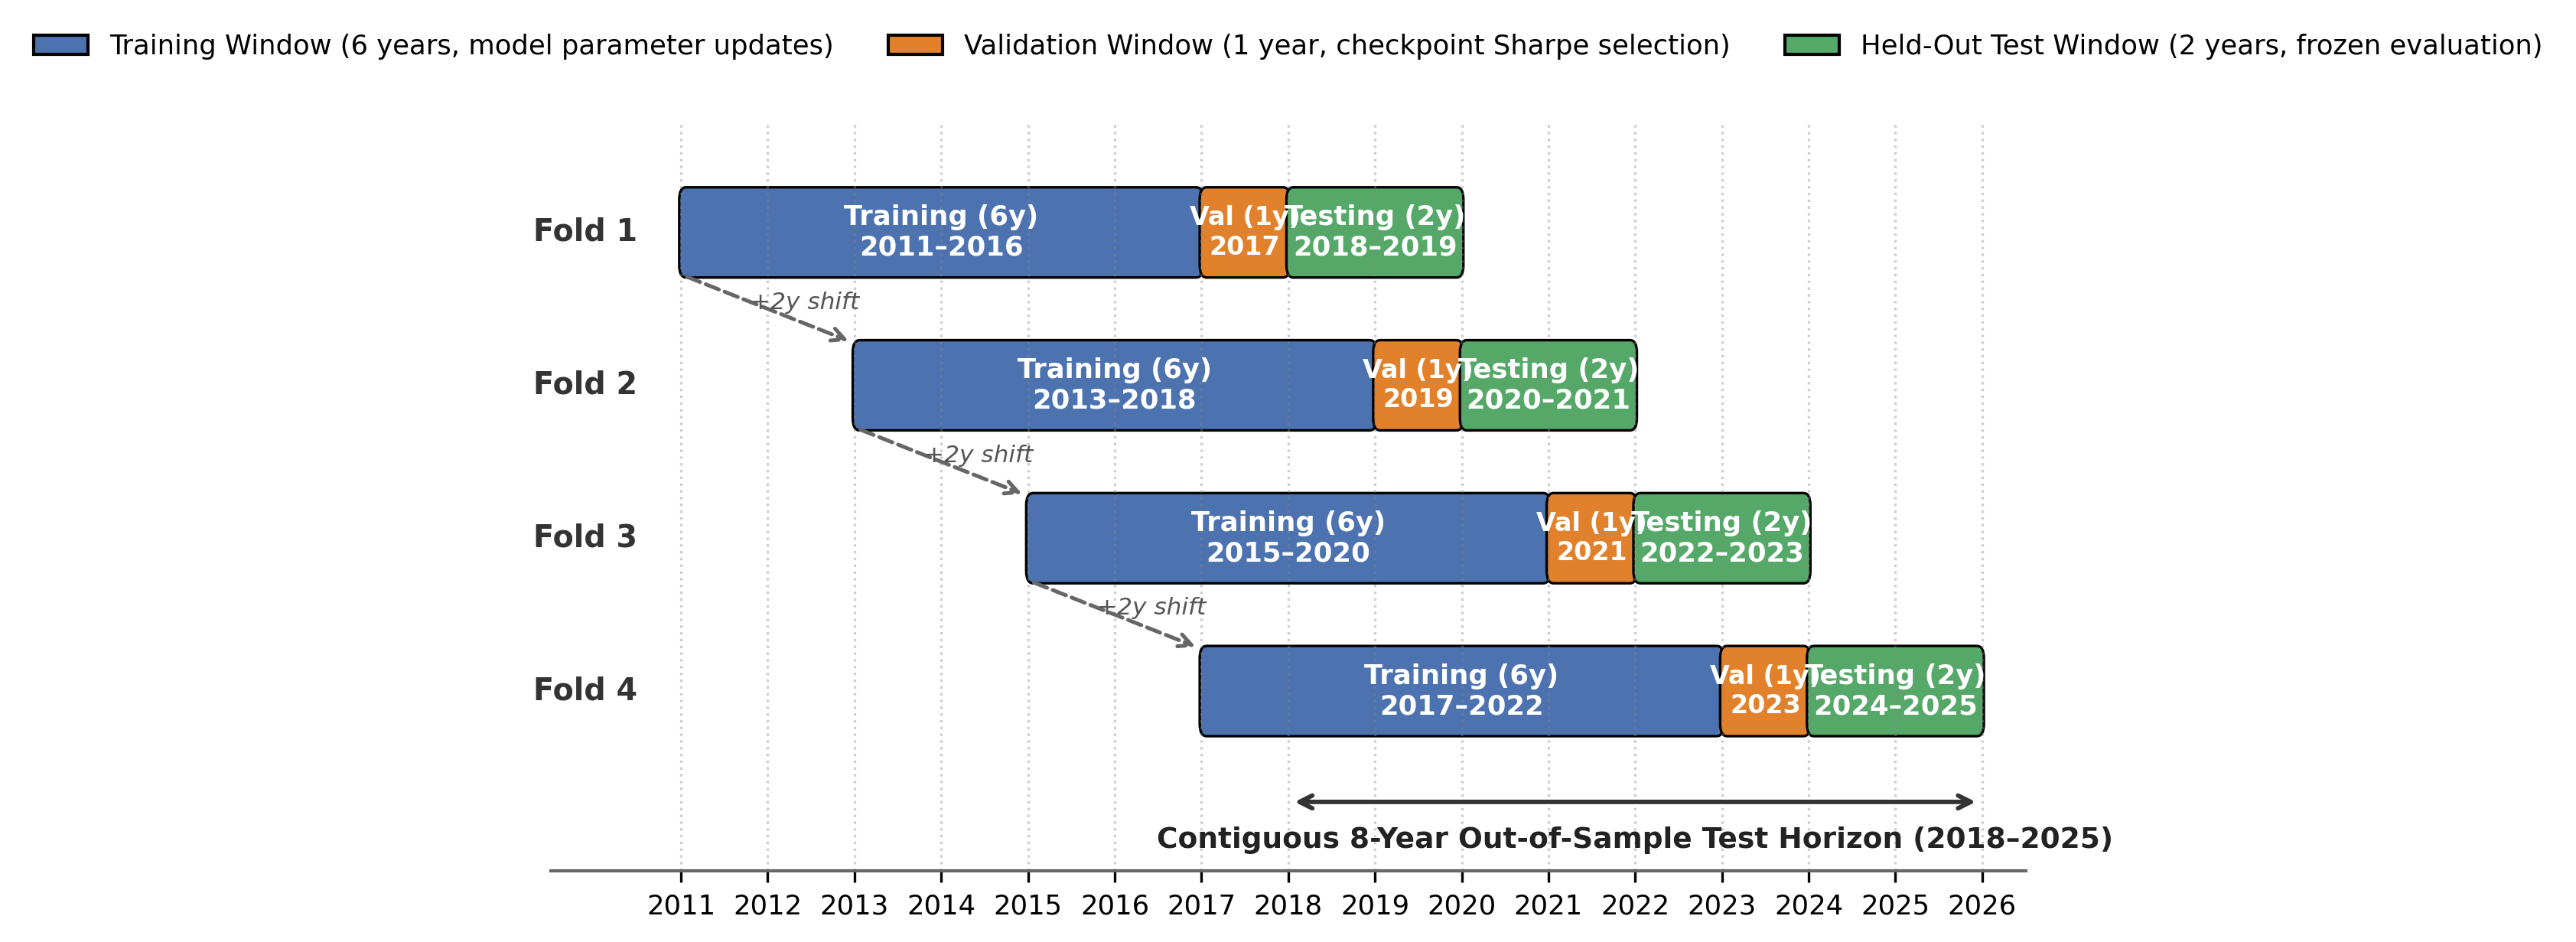
\includegraphics[width=0.92\textwidth]{figures/walk_forward_schematic.png}
\caption{Chronological four-fold rolling walk-forward evaluation protocol with 6-year training, 1-year validation, and 2-year testing windows, advancing by 2 years per fold (adapted from Liu et al. (2024), Figure 5).}
\label{fig:walk_forward}
\end{figure}

To assess statistical variability, each configuration is trained across three fixed random seeds ($S \in \{0, 1, 2\}$). During training, validation Sharpe ratio is evaluated periodically every 25,000 environment steps, and the checkpoint achieving the highest validation Sharpe ratio is saved. At the conclusion of 300,000 steps, this best-validation checkpoint is restored and evaluated once on the out-of-sample test window. 

\textit{Methodological Disclosure:} We note that earlier exploratory runs of Model M1 were conducted on Fold 1 test data during preliminary system debugging. We distinguish those preliminary debugging iterations from the final reported runs; test-set feedback was not used to adjust hyperparameters or select architectures.

\chapter{Model Architecture and Mathematical Formulation}
\label{ch:methodology}

\section{Overview of the Actor--Critic Architecture}
The portfolio management policy is trained using Proximal Policy Optimisation (PPO) \citep{schulman2017proximal} formulated within an Actor--Critic framework. The system architecture decouples temporal representation learning, continuous allocation policy parameterisation on the simplex manifold, and state-value baseline estimation:
\begin{enumerate}
    \item An \textbf{Encoder} processes the state observation to generate a compact 512-dimensional latent representation $\mathbf{h}_t \in \mathbb{R}^{512}$.
    \item An \textbf{Actor head} maps $\mathbf{h}_t$ to the parameters of a multivariate Dirichlet distribution that outputs portfolio allocations across $M = 11$ assets (10 equities plus cash).
    \item A \textbf{Critic head} maps $\mathbf{h}_t$ to a scalar baseline estimate $V_\phi(\mathbf{s}_t) \in \mathbb{R}$ approximating the expected cumulative discounted future reward.
\end{enumerate}

Figure~\ref{fig:architecture} illustrates the end-to-end information flow, and Figure~\ref{fig:pipeline} portrays the rollout interaction and PPO optimization pipeline.

\begin{figure}[htbp]
\centering
\begin{minipage}{0.49\textwidth}
\centering
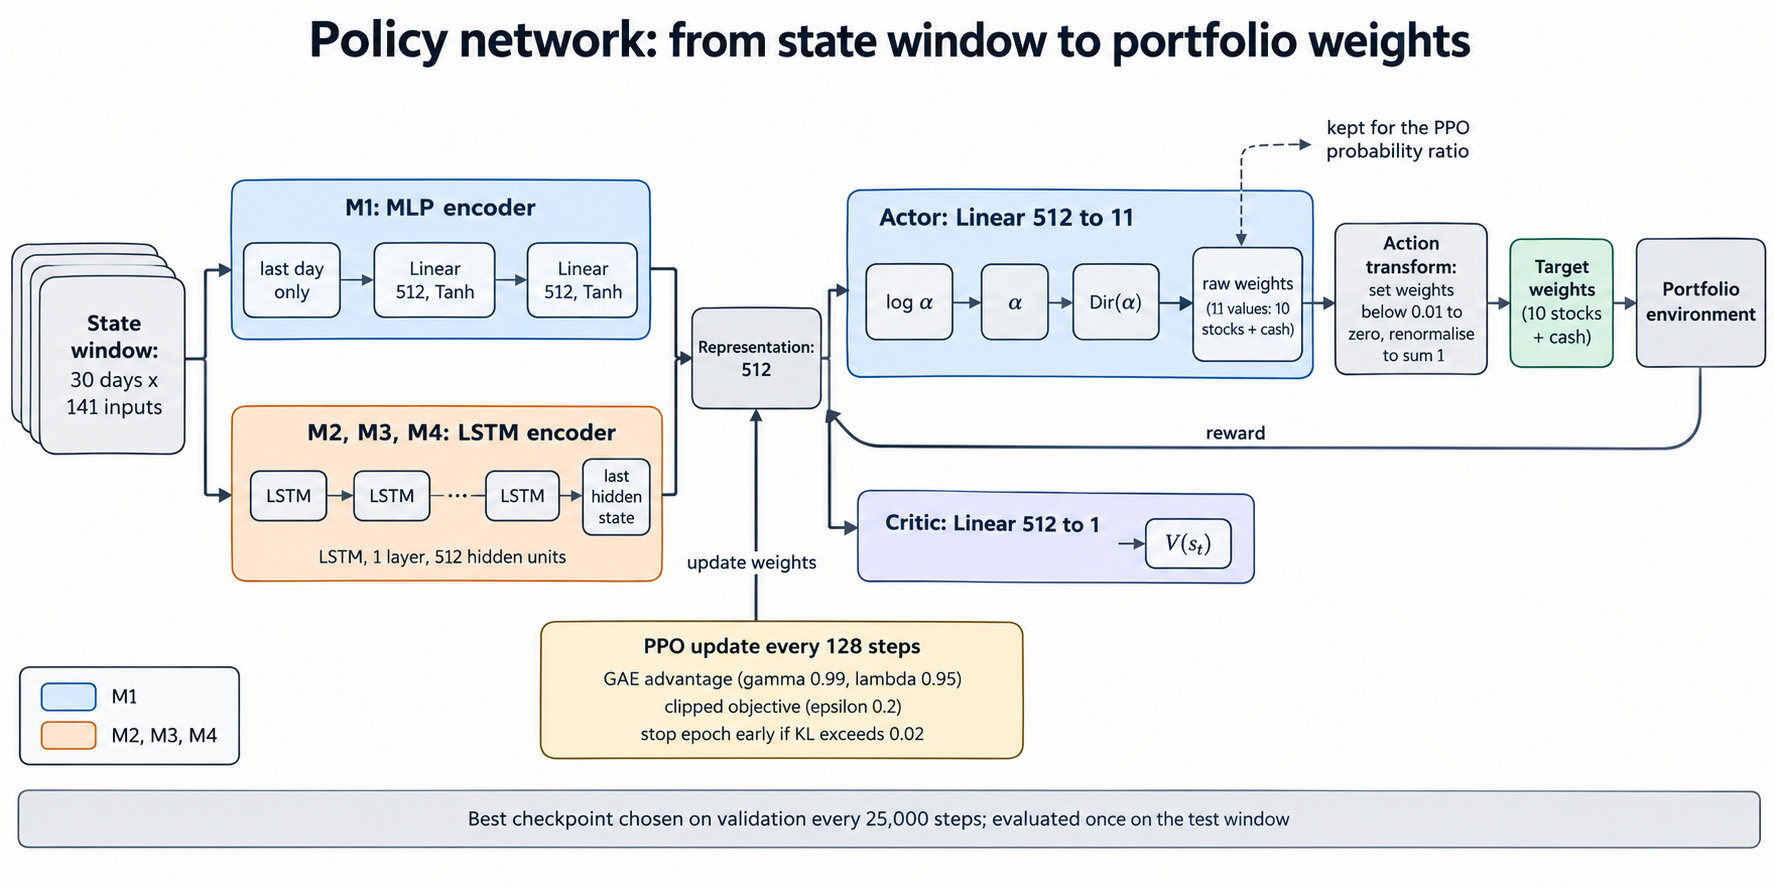
\includegraphics[width=\textwidth]{architecture.png}
\caption{Policy architecture from state to portfolio weights.}
\label{fig:architecture}
\end{minipage}\hfill
\begin{minipage}{0.49\textwidth}
\centering
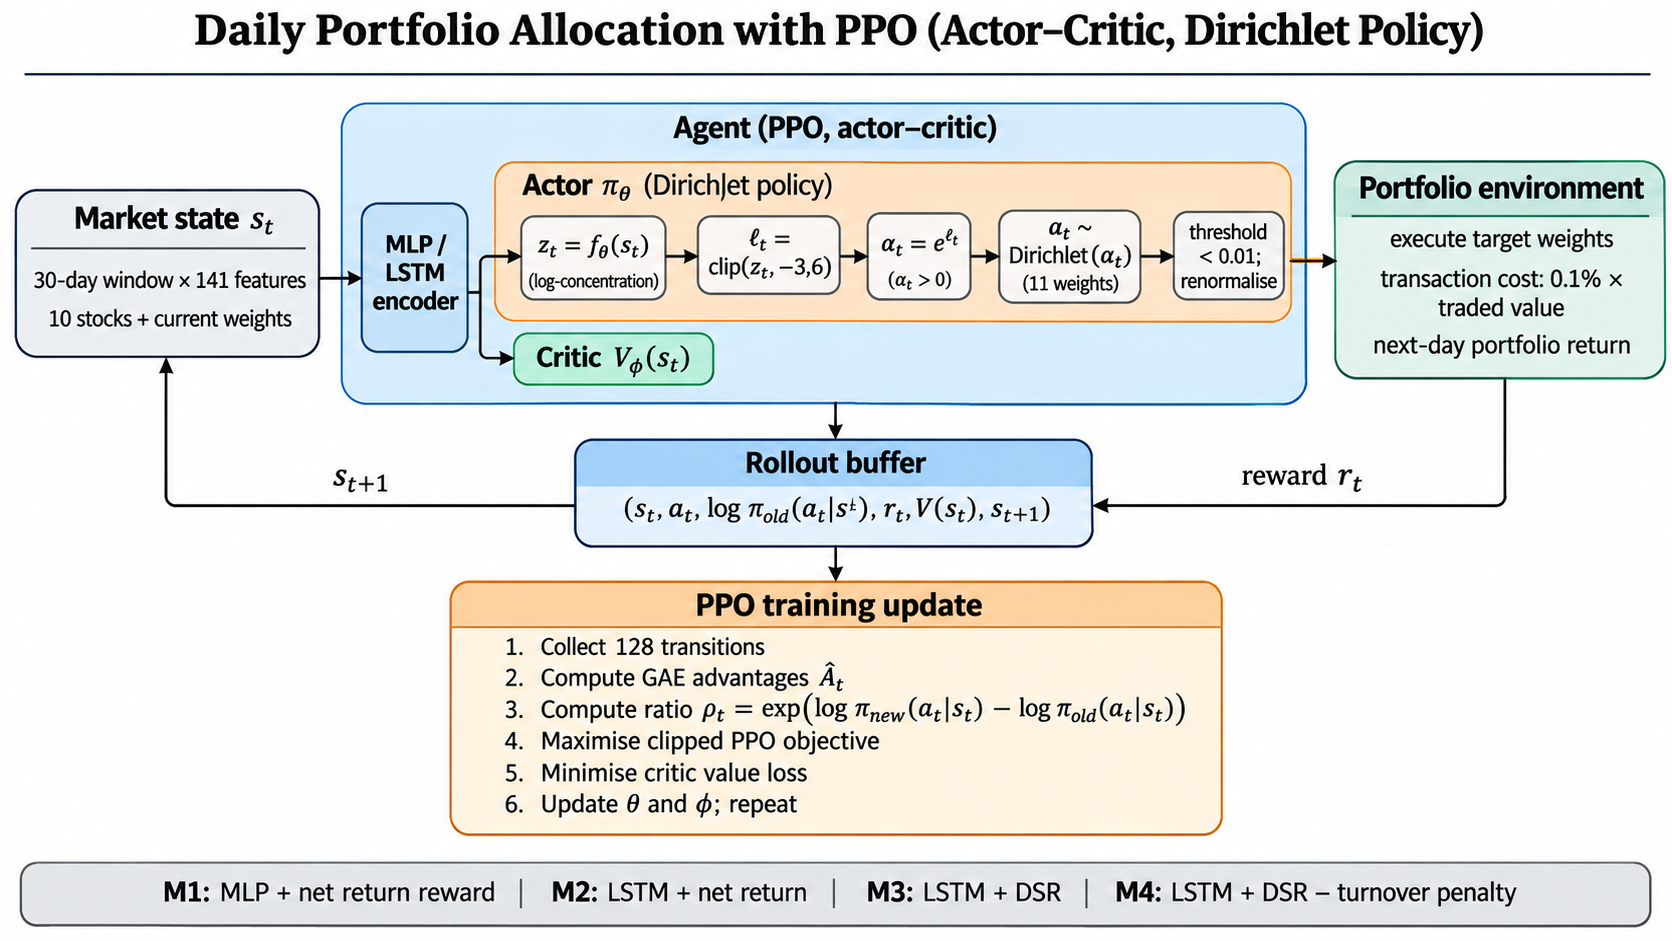
\includegraphics[width=\textwidth]{pipeline.png}
\caption{PPO Dirichlet allocation and environment loop.}
\label{fig:pipeline}
\end{minipage}
\end{figure}

\section{State Encoders: MLP versus Recurrent LSTM}
To rigorously evaluate the utility of temporal memory, two alternative encoder backbones are examined:

\subsection{Multi-Layer Perceptron (MLP) Encoder (Model M1)}
The feedforward MLP baseline observes solely the instantaneous observation vector at day $t$, $\mathbf{x}_t = \mathbf{s}_t \in \mathbb{R}^{141}$, discarding multi-period historical trajectories. The representation $\mathbf{h}_t$ is computed via two fully-connected layers with Tanh activations:
\begin{equation}
\mathbf{h}_t = \tanh\left( \mathbf{W}_2 \tanh\left( \mathbf{W}_1 \mathbf{x}_t + \mathbf{b}_1 \right) + \mathbf{b}_2 \right),
\end{equation}
where $\mathbf{W}_1 \in \mathbb{R}^{512 \times 141}$ and $\mathbf{W}_2 \in \mathbb{R}^{512 \times 512}$.

\subsection{Recurrent LSTM Encoder (Models M2--M4)}
To capture sequential price momentum and multi-period dependencies, Models M2, M3, and M4 pass the sliding history window $\mathbf{F}_t = [\mathbf{s}_{t-W+1}, \dots, \mathbf{s}_t] \in \mathbb{R}^{W \times 141}$ ($W = 30$) through a recurrent Long Short-Term Memory (LSTM) network:
\begin{equation}
(\mathbf{h}_t, \mathbf{c}_t) = \text{LSTM}(\mathbf{F}_t),
\end{equation}
with hidden representation size $H = 512$, following the empirical findings of \citet{zou2023novel}. The LSTM is trained end-to-end with the policy and value networks; rather than serving as an explicit price forecaster, $\mathbf{h}_t$ serves as a learned temporal belief state for sequential allocation.

\section{Continuous Dirichlet Policy on the Simplex}
\label{sec:dirichlet_policy}
A fundamental challenge in continuous portfolio control is ensuring that allocated asset weights satisfy the portfolio simplex constraints:
\begin{equation}
w_{i,t}^{\text{target}} \ge 0, \quad w_{\text{cash},t}^{\text{target}} \ge 0, \quad \sum_{i=1}^{N} w_{i,t}^{\text{target}} + w_{\text{cash},t}^{\text{target}} = 1.
\end{equation}
Following \citet{yang2022selective}, the policy is parameterised using a multivariate Dirichlet distribution, which natively defines a probability measure directly over the open unit simplex without requiring arbitrary heuristic projections.

\subsection{Actor Mapping to Dirichlet Parameters}
The actor network maps the latent representation $\mathbf{h}_t$ to an unconstrained linear vector $\mathbf{z}_t \in \mathbb{R}^{N+1}$:
\begin{equation}
\mathbf{z}_t = \mathbf{W}_a \mathbf{h}_t + \mathbf{b}_a, \quad \mathbf{W}_a \in \mathbb{R}^{(N+1) \times 512}, \; \mathbf{b}_a \in \mathbb{R}^{N+1}.
\end{equation}
To ensure numerical stability during gradient backpropagation, the outputs are clamped to a safe log-concentration range and exponentiated to yield strictly positive Dirichlet concentration parameters $\boldsymbol{\alpha}_t \in \mathbb{R}_{>0}^{N+1}$:
\begin{align}
\boldsymbol{\ell}_t &= \text{clip}\left( \mathbf{z}_t, -3.0, 6.0 \right), \\
\alpha_{i,t} &= \exp\left( \ell_{i,t} \right) \in \left[ e^{-3}, e^6 \right] \approx [0.0498, 403.43].
\end{align}
Clamping prevents underflow (which leads to degenerate distributions concentrated at vertices) and overflow (which causes numerical instability in the Gamma function derivative).

\subsection{Action Sampling and Expected Allocation}
The continuous action $\mathbf{a}_t \in \Delta^N$ is sampled from the Dirichlet probability density:
\begin{equation}
\label{eq:dirichlet_pdf}
\pi_\theta(\mathbf{a}_t \mid \mathbf{h}_t) = \frac{\Gamma\left( \sum_{i=1}^{N+1} \alpha_{i,t} \right)}{\prod_{i=1}^{N+1} \Gamma(\alpha_{i,t})} \prod_{i=1}^{N+1} a_{i,t}^{\alpha_{i,t} - 1},
\end{equation}
where $\Gamma(z)$ is the standard Gamma function. Sampling is performed via normalized independent Gamma variates: $g_{i,t} \sim \text{Gamma}(\alpha_{i,t}, 1)$ with $a_{i,t} = g_{i,t} / \sum_j g_{j,t}$. The expected portfolio allocation is:
\begin{equation}
\mathbb{E}\left[ a_{i,t} \right] = \frac{\alpha_{i,t}}{\sum_{j=1}^{N+1} \alpha_{j,t}}.
\end{equation}
During deterministic out-of-sample evaluation, the policy executes this expected allocation directly.

\subsection{Sparsity Thresholding and Renormalisation}
Because a Dirichlet distribution with positive parameters assigns non-zero mass across all assets, raw samples can contain minuscule allocations (e.g., $0.05\%$) that induce unneeded rebalancing fees. A threshold $\tau = 0.01$ (1\%) is applied identically across all models:
\begin{equation}
\label{eq:thresholding}
\tilde{w}_{i,t} = 
\begin{cases}
a_{i,t}, & \text{if } a_{i,t} \ge \tau, \\
0, & \text{if } a_{i,t} < \tau,
\end{cases}
\qquad
w_{i,t}^{\text{target}} = \frac{\tilde{w}_{i,t}}{\sum_{j=1}^{N+1} \tilde{w}_{j,t}}.
\end{equation}
This operation liquidates tiny positions and renormalises the surviving allocations to sum strictly to one.

\section{Portfolio Dynamics and Transaction Cost Accounting}
Let $\mathbf{w}_t^{\text{cur}} \in \Delta^N$ denote the portfolio weights immediately preceding rebalancing at day $t$. The required reallocation across the risky equities is $\Delta w_{i,t} = w_{i,t}^{\text{target}} - w_{i,t}^{\text{cur}}$.

Reallocating between cash and risky assets incurs a proportional transaction fee $c_{\text{trans}} = 0.001$ ($10\text{ bps}$):
\begin{equation}
C_t = c_{\text{trans}} V_{t-1} \sum_{i=1}^N \left| \Delta w_{i,t} \right|.
\end{equation}
End-of-day portfolio wealth $V_t$ evolves according to:
\begin{equation}
V_t = (V_{t-1} - C_t) \left[ \sum_{i=1}^N w_{i,t}^{\text{target}} (1 + R_{i,t}) + w_{\text{cash},t}^{\text{target}} \right],
\end{equation}
where $R_{i,t} = \frac{C_{i,t}}{C_{i,t-1}} - 1$ is the simple price return. The net portfolio return used throughout the framework is:
\begin{equation}
R_{\text{net},t} = \frac{V_t - V_{t-1}}{V_{t-1}}.
\end{equation}

\section{Model Reward Formulations (M1 to M4)}
The reward signal $r_t$ emitted to the agent constitutes the core ablation dimension:
\begin{enumerate}
    \item \textbf{Models M1 and M2 (Net Return Reward):}
    \begin{equation}
    r_t = R_{\text{net},t}.
    \end{equation}

    \item \textbf{Model M3 (Differential Sharpe Ratio):}
    Following \citet{millea2021deep}, an online recursive Differential Sharpe Ratio (DSR) is computed without requiring batch return histories. Moving estimates of the first and second return moments ($A_t \approx \mathbb{E}[R]$ and $B_t \approx \mathbb{E}[R^2]$) update exponentially with adaptation rate $\eta = 0.01$:
    \begin{align}
    A_t &= A_{t-1} + \eta (R_{\text{net},t} - A_{t-1}), \\
    B_t &= B_{t-1} + \eta (R_{\text{net},t}^2 - B_{t-1}).
    \end{align}
    With moment changes $\Delta A_t = A_t - A_{t-1}$ and $\Delta B_t = B_t - B_{t-1}$, the DSR reward is:
    \begin{equation}
    D_t = \frac{B_{t-1} \Delta A_t - \frac{1}{2} A_{t-1} \Delta B_t}{\left( B_{t-1} - A_{t-1}^2 + \varepsilon_{\text{DSR}} \right)^{3/2}},
    \end{equation}
    where $\varepsilon_{\text{DSR}} = 10^{-8}$ prevents numerical division by zero. For Model M3, $r_t = D_t$.

    \item \textbf{Model M4 (DSR with Squared Turnover Penalty):}
    To discourage excessive daily weight churn, an explicit quadratic turnover penalty is subtracted from the DSR reward:
    \begin{equation}
    r_t = D_t - \lambda_{\text{turn}} \sum_{i=1}^N \left( w_{i,t}^{\text{target}} - w_{i,t}^{\text{cur}} \right)^2,
    \end{equation}
    with $\lambda_{\text{turn}} = 0.1$ selected via validation tuning.
\end{enumerate}

\section{PPO Policy Optimisation}
During environment interaction, the agent collects transitions and stores the raw sampled continuous action $\mathbf{a}_t$ along with its log-likelihood under old parameters $\theta_{\text{old}}$:
\begin{equation}
\log \pi_{\theta_{\text{old}}}(\mathbf{a}_t \mid \mathbf{h}_t) = \ln \Gamma\left( \sum_{i=1}^{N+1} \alpha_{i,t} \right) - \sum_{i=1}^{N+1} \ln \Gamma(\alpha_{i,t}) + \sum_{i=1}^{N+1} (\alpha_{i,t} - 1) \ln a_{i,t}.
\end{equation}

Generalized Advantage Estimation (GAE) computes advantages $\hat{A}_t$ using temporal-difference residuals $\delta_t = \tilde{r}_t + \gamma V_\phi(\mathbf{s}_{t+1}) - V_\phi(\mathbf{s}_t)$ with discount $\gamma = 0.99$ and trace decay $\lambda_{\text{GAE}} = 0.95$:
\begin{equation}
\hat{A}_t = \sum_{l=0}^\infty (\gamma \lambda_{\text{GAE}})^l \delta_{t+l}.
\end{equation}

During mini-batch optimisation, the probability ratio is evaluated for the identical raw action $\mathbf{a}_t$:
\begin{equation}
\rho_t(\theta) = \frac{\pi_\theta(\mathbf{a}_t \mid \mathbf{h}_t)}{\pi_{\theta_{\text{old}}}(\mathbf{a}_t \mid \mathbf{h}_t)} = \exp\left( \log \pi_\theta(\mathbf{a}_t \mid \mathbf{h}_t) - \log \pi_{\theta_{\text{old}}}(\mathbf{a}_t \mid \mathbf{h}_t) \right).
\end{equation}
The policy parameters $\theta$ and critic parameters $\phi$ are updated by minimising the joint multi-task loss \citep{schulman2017proximal}:
\begin{equation}
\mathcal{L}(\theta, \phi) = -\hat{\mathbb{E}}_t \left[ \min\left( \rho_t(\theta) \hat{A}_t, \; \text{clip}(\rho_t(\theta), 1 - \epsilon, 1 + \epsilon) \hat{A}_t \right) \right] + c_1 \hat{\mathbb{E}}_t \left[ (V_\phi(\mathbf{s}_t) - \hat{V}_t^{\text{target}})^2 \right] - c_2 \hat{\mathbb{E}}_t [\mathcal{H}(\pi_\theta)],
\end{equation}
with clipping range $\epsilon = 0.2$, critic weight $c_1 = 0.5$, and entropy bonus $c_2 = 0.01$.

\begin{figure}[htbp]
\centering
\begin{minipage}{0.96\textwidth}
\hrule \vspace{2pt} \hrule \vspace{4pt}
\noindent\textbf{Algorithm 1: PPO Daily Portfolio Allocation with Dirichlet Policy}
\vspace{4pt} \hrule \vspace{6pt}
\footnotesize
\noindent\textbf{Input:} Market series $\mathbf{X}$, returns $\mathbf{R}$, cost $c_{\text{trans}}$, threshold $\tau$, penalty $\lambda_{\text{turn}}$, PPO parameters $\gamma, \lambda_{\text{GAE}}, \epsilon, \eta_{\text{LR}}$.\\
\textbf{Initialisation:} Actor $\theta$, Critic $\phi$, reward normaliser $\mathcal{N}$, initial weights $\mathbf{w}_0^{\text{cur}} \gets [0, \dots, 0, 1]^\top$ (cash), DSR moments $A \gets 0, B \gets 0$.
\vspace{4pt}
\begin{enumerate}
    \item \textbf{for} $\text{iteration} = 1, 2, \dots$ until $T_{\text{total}} = 300,000$ steps \textbf{do}
    \item \quad Reset rollout buffer $\mathcal{B} \gets \emptyset$.
    \item \quad \textbf{for} $t = 1$ to $T_{\text{rollout}} = 128$ \textbf{do}
    \item \qquad Compute representation $\mathbf{h}_t \gets \text{Encoder}(\mathbf{s}_t)$ (MLP for M1; LSTM for M2--M4).
    \item \qquad Compute concentrations $\boldsymbol{\ell}_t \gets \text{clip}(\mathbf{W}_a \mathbf{h}_t + \mathbf{b}_a, -3, 6)$ and $\boldsymbol{\alpha}_t \gets \exp(\boldsymbol{\ell}_t)$.
    \item \qquad Sample raw action variates $g_i \sim \text{Gamma}(\alpha_{i,t}, 1)$, set $\mathbf{a}_t \gets \mathbf{g} / \sum_i g_i$.
    \item \qquad Evaluate old log-likelihood $lp_t \gets \log \pi_\theta(\mathbf{a}_t \mid \mathbf{h}_t)$ and value $V_t \gets V_\phi(\mathbf{h}_t)$.
    \item \qquad Apply threshold $\tau = 0.01$: $\tilde{w}_i \gets a_{i,t} \cdot \mathbf{1}_{a_{i,t} \ge \tau}$, set $\mathbf{w}_t^{\text{target}} \gets \tilde{\mathbf{w}} / \sum_j \tilde{w}_j$.
    \item \qquad Execute trade: compute $\text{Turnover}_t$, cost $C_t$, net return $R_{\text{net},t}$, new wealth $V_t$.
    \item \qquad Compute model reward $r_t$ (Net return for M1/M2; DSR for M3; DSR $-\lambda_{\text{turn}} \sum (\Delta w_i)^2$ for M4).
    \item \qquad Store transition $(\mathbf{s}_t, \mathbf{a}_t, lp_t, V_t, r_t)$ in buffer $\mathcal{B}$.
    \item \quad \textbf{end for}
    \item \quad Compute GAE advantages $\hat{A}_t$ and return targets $\hat{V}_t^{\text{target}}$.
    \item \quad \textbf{for} $\text{epoch} = 1$ to $K = 10$ \textbf{do}
    \item \qquad \textbf{for} each minibatch of size $B = 64$ \textbf{do}
    \item \qquad\quad Evaluate current log-likelihoods $\log \pi_\theta(\mathbf{a}_i \mid \mathbf{h}_i)$ and values $V_\phi(\mathbf{h}_i)$.
    \item \qquad\quad Compute probability ratio $\rho_i(\theta) \gets \exp(\log \pi_\theta - lp_i)$ and multi-task loss $\mathcal{L}(\theta, \phi)$.
    \item \qquad\quad Update $(\theta, \phi)$ via Adam optimiser ($\eta_{\text{LR}} = 10^{-4}$) with gradient clipping $0.5$.
    \item \qquad \textbf{end for}
    \item \quad \textbf{end for}
    \item \textbf{end for}
\end{enumerate}
\vspace{4pt} \hrule
\end{minipage}
\caption{Complete training and policy update algorithm for PPO portfolio allocation.}
\label{alg:ppo_portfolio}
\end{figure}

\chapter{Controlled Ablation Study Design}
\label{ch:ablation}

\section{Specification of Ablation Models M1--M4}
To evaluate the contribution of each algorithmic component without confounding factors, we adopt a single-factor ablation design. Four model configurations (M1 through M4) are specified such that each successive transition alters exactly one algorithmic mechanism while holding all other parameters, training budgets, random seeds, transaction costs, and data folds strictly invariant:
\begin{enumerate}
    \item \textbf{Model M1 (MLP Baseline + Net Return):} Two-layer feedforward MLP observing solely instantaneous market observation $\mathbf{s}_t \in \mathbb{R}^{141}$ with net return reward ($r_t = R_{\text{net},t}$) and zero penalty ($\lambda_{\text{turn}} = 0$).
    \item \textbf{Model M2 (LSTM Recurrent Encoder + Net Return):} Replaces the static MLP with a single-layer LSTM ($H=512$) over sliding window $\mathbf{F}_t \in \mathbb{R}^{30 \times 141}$. Reward remains net return ($r_t = R_{\text{net},t}$). Transition M1 $\to$ M2 isolates \textbf{temporal memory and sequence modeling}.
    \item \textbf{Model M3 (LSTM Encoder + Differential Sharpe Ratio):} Retains the LSTM backbone, replacing net return with the recursive Differential Sharpe Ratio ($r_t = D_t$). Transition M2 $\to$ M3 isolates \textbf{risk-aware reward engineering}.
    \item \textbf{Model M4 (LSTM + DSR + Quadratic Turnover Regularisation):} Retains the LSTM backbone and DSR reward, augmented by a quadratic weight-change penalty on risky assets ($r_t = D_t - \lambda_{\text{turn}} \sum_{j=1}^{10} (w_{j,t}^{\text{target}} - w_{j,t}^{\text{cur}})^2$) with $\lambda_{\text{turn}} = 0.1$. Transition M3 $\to$ M4 isolates \textbf{turnover regularisation}.
\end{enumerate}

Table~\ref{tab:ablation_matrix} summarises the systematic ablation matrix across all four configurations.

\begin{table}[htbp]
\centering
\scriptsize
\setlength{\tabcolsep}{3pt}
\caption{Systematic ablation matrix across models M1 to M4.}
\label{tab:ablation_matrix}
\begin{tabular}{lcccc}
\toprule
\textbf{Configuration Property} & \textbf{Model M1} & \textbf{Model M2} & \textbf{Model M3} & \textbf{Model M4} \\
\midrule
Encoder Backbone & MLP (2-layer) & LSTM (1-layer) & LSTM (1-layer) & LSTM (1-layer) \\
Temporal Window ($T$) & 1 day (last row) & 30 days & 30 days & 30 days \\
Latent Dimension ($H$) & 512 & 512 & 512 & 512 \\
Policy Head & Dirichlet $\Delta^{10}$ & Dirichlet $\Delta^{10}$ & Dirichlet $\Delta^{10}$ & Dirichlet $\Delta^{10}$ \\
Action Threshold ($\tau$) & 0.01 & 0.01 & 0.01 & 0.01 \\
Reward Formulation & Net Return & Net Return & DSR ($D_t$) & DSR ($D_t$) \\
Turnover Regularisation & None ($\lambda = 0$) & None ($\lambda = 0$) & None ($\lambda = 0$) & Quadratic Penalty ($\lambda = 0.1$) \\
Environment Cost Model & $0.1\%$ per turnover & $0.1\%$ per turnover & $0.1\%$ per turnover & $0.1\%$ per turnover \\
Training Budget & 300,000 steps & 300,000 steps & 300,000 steps & 300,000 steps \\
\midrule
\textbf{Ablation Mechanism} & \textit{Baseline} & \textbf{+ Temporal} & \textbf{+ Risk-Aware} & \textbf{+ Turnover Penalty} \\
\bottomrule
\end{tabular}
\end{table}

\section{Control Invariants and Training Algorithm}
Experimental controls are strictly enforced: (i)~Actor and Critic heads are instantiated prior to the encoder to ensure identical initial head weights across models under the same seed; (ii)~all models train for exactly 300,000 steps with identical Adam learning rate ($10^{-4}$), rollout horizon (128), and batch size (64); (iii)~all models experience identical market sequences and transaction costs; and (iv)~programmatic assertions verify that each transition alters exactly one dimension. Algorithm~\ref{alg:ppo_portfolio} details the training workflow.

\begin{figure}[htbp]
\centering
\begin{minipage}{0.98\textwidth}
\hrule \vspace{2pt} \hrule \vspace{3pt}
\noindent\textbf{Algorithm 1: Continuous Dirichlet PPO Daily Portfolio Allocation}
\vspace{3pt} \hrule \vspace{4pt}
\scriptsize
\textbf{Input:} Market indicators $\mathbf{X}$, returns $\mathbf{R}$, cost $c_{\text{trans}} = 0.001$, threshold $\tau = 0.01$, penalty $\lambda_{\text{turn}}$, PPO hyperparameters ($\gamma, \lambda_{\text{GAE}}, \epsilon, \eta = 10^{-4}$).\\
\textbf{Output:} Optimised policy weights $\theta^*$ selected by peak validation Sharpe ratio.\\[2pt]
\textbf{Initialisation:} Initialise shared Encoder, Actor $\theta$, Critic $\phi$, Adam optimiser; $V_0 \gets 10^6$, $\mathbf{w}_0^{\text{cur}} \gets [0,\dots,0,1]^\top$; DSR moments $A_0 \gets 0, B_0 \gets 0$; step counter $N_{\text{step}} \gets 0$, $SR_{\text{best}} \gets -\infty$.\\[2pt]
\textbf{Procedure:}
\begin{enumerate}[1:]
    \setlength{\itemsep}{0.5pt}
    \item \textbf{while} $N_{\text{step}} < 300{,}000$ \textbf{do}
    \item \quad Reset rollout buffer $\mathcal{B} \gets \emptyset$.
    \item \quad \textbf{for} $t = 1$ \textbf{to} $T_{\text{rollout}} = 128$ \textbf{do}
    \item \qquad Compute $\mathbf{h}_t \gets \text{Encoder}(\mathbf{s}_t)$ (or $\mathbf{F}_t$), $\boldsymbol{\ell}_t \gets \operatorname{clip}(\mathbf{W}_a \mathbf{h}_t + \mathbf{b}_a, -3, 6)$, and $\boldsymbol{\alpha}_t \gets \exp(\boldsymbol{\ell}_t)$.
    \item \qquad Sample raw continuous action $\mathbf{a}_t \sim \operatorname{Dirichlet}(\boldsymbol{\alpha}_t)$; record $lp_t \gets \log \pi_\theta(\mathbf{a}_t \mid \mathbf{s}_t)$ and $V_t \gets V_\phi(\mathbf{s}_t)$.
    \item \qquad Apply threshold: $\tilde{w}_{i,t} \gets a_{i,t} \cdot \mathbf{1}_{a_{i,t} \ge \tau}$; set target weights $\mathbf{w}_t^{\text{target}} \gets \tilde{\mathbf{w}}_t / \sum_j \tilde{w}_{j,t}$.
    \item \qquad Rebalance: $\text{Turnover}_t \gets \sum_{i=1}^{10} |w_{i,t}^{\text{target}} - w_{i,t}^{\text{cur}}|$, fee $C_t \gets c_{\text{trans}} V_t \text{Turnover}_t$.
    \item \qquad Advance environment: update wealth $V_{t+1}$, net return $R_{\text{net},t} \gets (V_{t+1}-V_t)/V_t$, and drifted weights $\mathbf{w}_{t+1}^{\text{cur}}$.
    \item \qquad Compute model reward: $r_t \gets R_{\text{net},t}$ (M1, M2); $r_t \gets D_t$ (M3); $r_t \gets D_t - \lambda_{\text{turn}}\sum_{i=1}^{10} (w_{i,t}^{\text{target}}-w_{i,t}^{\text{cur}})^2$ (M4).
    \item \qquad Store $(\mathbf{s}_t, \mathbf{a}_t, lp_t, V_t, r_t)$ in $\mathcal{B}$; $N_{\text{step}} \gets N_{\text{step}} + 1$.
    \item \quad \textbf{end for}
    \item \quad Standardise rewards, compute GAE advantages $\hat{A}_t$ and returns $\hat{V}_t^{\text{target}}$.
    \item \quad \textbf{for} $\text{epoch} = 1$ \textbf{to} $10$ \textbf{do}
    \item \qquad \textbf{for} each mini-batch $B = 64$ from $\mathcal{B}$ \textbf{do}
    \item \qquad\quad Evaluate ratio $\rho_i(\theta) \gets \exp(\log \pi_\theta - lp_i)$ and approximate KL divergence; break if $\text{KL} > 0.03$.
    \item \qquad\quad Update $(\theta, \phi)$ via Adam ($\eta = 10^{-4}$, grad clip $0.5$) using total loss $\mathcal{L}^{\text{total}}(\theta, \phi)$ (Eq.~\eqref{eq:total_loss}).
    \item \qquad \textbf{end for}
    \item \quad \textbf{end for}
    \item \quad \textbf{if} $N_{\text{step}} \pmod{25{,}000} = 0$ \textbf{then} evaluate $SR_{\text{val}}$; \textbf{if} $SR_{\text{val}} > SR_{\text{best}}$ \textbf{then} save checkpoint $\theta^* \gets \theta$ \textbf{end if}
    \item \textbf{end while}
    \item Restore best checkpoint $\theta^*$ for final out-of-sample test evaluation.
\end{enumerate}
\vspace{1pt} \hrule
\end{minipage}
\caption{Complete PPO training algorithm for continuous Dirichlet portfolio allocation.}
\label{alg:ppo_portfolio}
\end{figure}

\chapter{Results and Discussion}
\label{ch:results}

\section{Overall Out-of-Sample Performance}
Out-of-sample evaluation was conducted across four chronological 2-year test segments spanning 2018 through 2025. Table~\ref{tab:overall_results} presents the pooled test performance metrics (averaged across four folds and three random seeds) for models M1--M4 alongside the passive Equal-Weight (EW) 1/N benchmark.

\begin{table}[htbp]
\centering
\footnotesize
\setlength{\tabcolsep}{3pt}
\caption{Pooled out-of-sample test performance across 4 folds and 3 seeds (mean $\pm$ standard deviation).}
\label{tab:overall_results}
\begin{tabular}{lcccccc}
\toprule
\textbf{Model} & \textbf{Cum. Return (\%)} & \textbf{CAGR (\%)} & \textbf{Sharpe Ratio} & \textbf{Sortino} & \textbf{Max DD (\%)} & \textbf{Cost (\% of $V_0$)} \\
\midrule
\textbf{M1 (MLP)} & $20.62 \pm 5.14$ & $9.90 \pm 2.31$ & $0.71 \pm 0.13$ & $1.03 \pm 0.20$ & $-19.50 \pm 1.04$ & $9.68 \pm 0.10$ \\
\textbf{M2 (LSTM)} & $28.23 \pm 2.03$ & $13.37 \pm 0.88$ & $0.92 \pm 0.07$ & $1.34 \pm 0.09$ & $-18.52 \pm 1.35$ & $4.27 \pm 1.44$ \\
\textbf{M3 (+ DSR)} & $26.93 \pm 3.27$ & $12.68 \pm 1.56$ & $0.92 \pm 0.11$ & $1.34 \pm 0.17$ & $-19.95 \pm 0.81$ & $4.14 \pm 1.15$ \\
\textbf{M4 (+ Turn. Pen.)} & $20.97 \pm 4.19$ & $10.09 \pm 1.85$ & $0.92 \pm 0.17$ & $1.37 \pm 0.26$ & $\mathbf{-16.04 \pm 1.72}$ & $\mathbf{0.97 \pm 0.15}$ \\
\midrule
\textbf{Equal-Weight} & $\mathbf{36.48}$ & $\mathbf{17.08}$ & $\mathbf{1.13}$ & $\mathbf{1.66}$ & $-18.91$ & $\mathbf{0.61}$ \\
\bottomrule
\end{tabular}
\end{table}

Figure~\ref{fig:equity_stitched} illustrates cumulative out-of-sample portfolio profit (assuming $V_0 = \text{INR } 1{,}000{,}000$ initial capital reinvested sequentially) across the continuous 2018--2025 timeline. Figure~\ref{fig:drawdown} portrays peak-to-trough drawdowns, and Figure~\ref{fig:profit_bars} depicts profit across each 2-year test window.

\begin{figure}[htbp]
\centering
\begin{minipage}{0.49\textwidth}
\centering
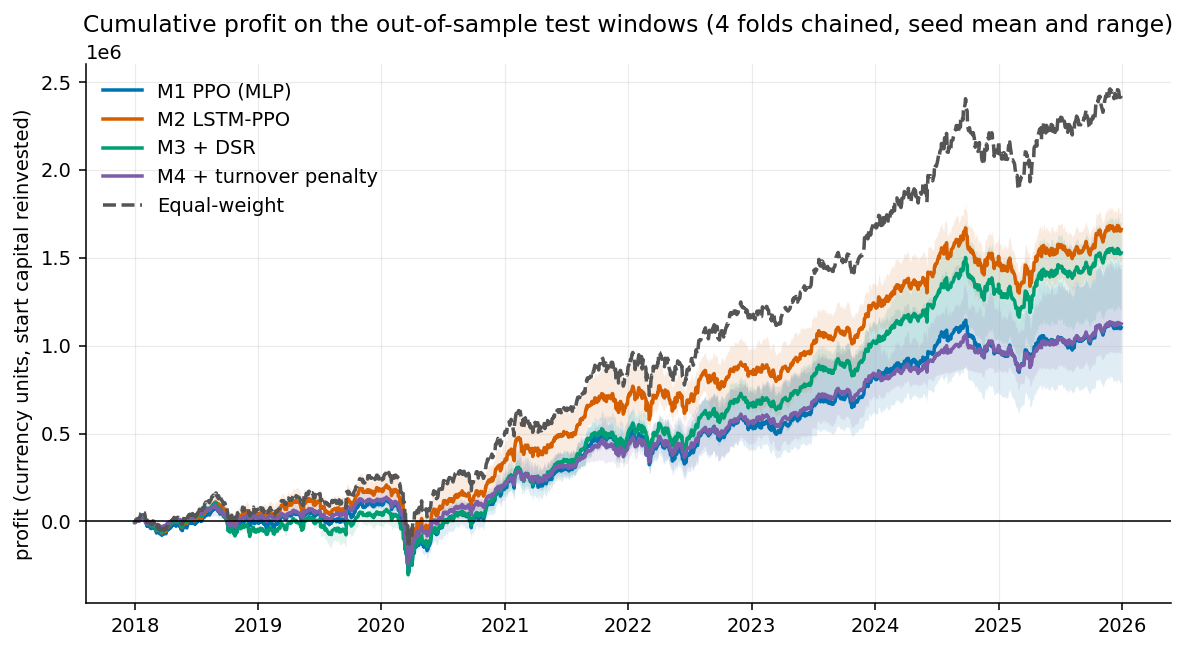
\includegraphics[width=\textwidth]{equity_stitched.png}
\caption{Cumulative out-of-sample profit across 4 chained test windows (2018--2025).}
\label{fig:equity_stitched}
\end{minipage}\hfill
\begin{minipage}{0.49\textwidth}
\centering
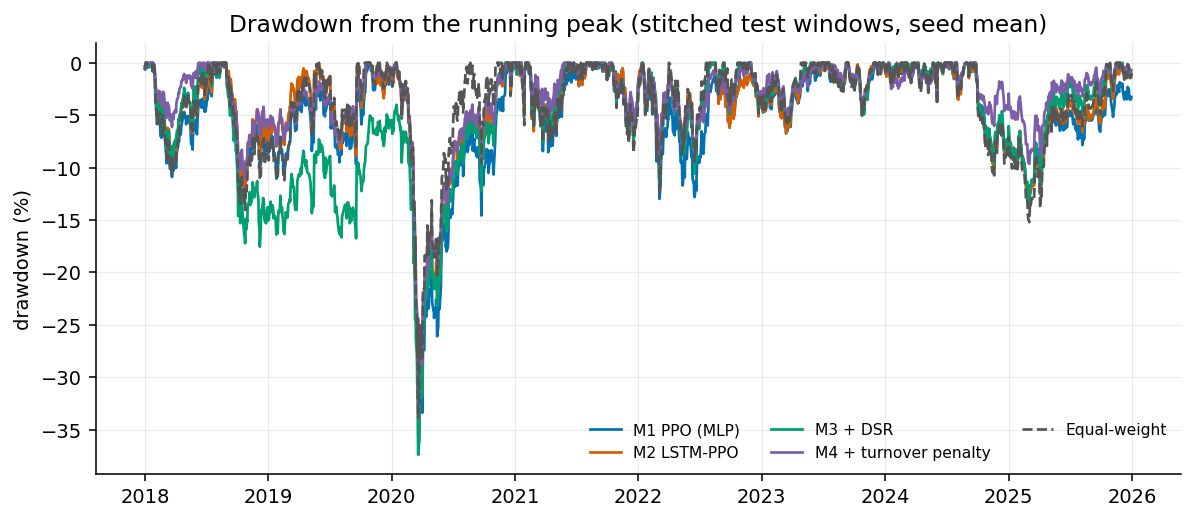
\includegraphics[width=\textwidth]{drawdown.png}
\caption{Out-of-sample portfolio drawdown from running peak (2018--2025).}
\label{fig:drawdown}
\end{minipage}
\end{figure}

\section{Analysis of Ablation Steps}
To establish statistical significance, paired difference tests were computed across all (fold, seed) tuples using 10,000-sample fold-level bootstrap resampling. Table~\ref{tab:ablation_deltas} reports the resulting paired deltas and 95\% confidence intervals.

\begin{table}[htbp]
\centering
\scriptsize
\setlength{\tabcolsep}{2.5pt}
\caption{Paired ablation differences ($b - a$) with 95\% bootstrap confidence intervals.}
\label{tab:ablation_deltas}
\begin{tabular}{llcccc}
\toprule
\textbf{Ablation Transition} & \textbf{Metric} & \textbf{Mean Delta} & \textbf{95\% CI} & \textbf{Folds Improved} & \textbf{Pairs Improved} \\
\midrule
\multirow{4}{*}{\textbf{M1 $\to$ M2} (Temporal Memory)} 
& Sharpe Ratio & $+0.201$ & $[+0.156, +0.246]$ & $4 / 4$ & $9 / 12$ \\
& Cum. Return (\%) & $+7.61\%$ & $[+4.81\%, +10.01\%]$ & $4 / 4$ & $10 / 12$ \\
& Daily Turnover & $-0.106$ & $[-0.138, -0.070]$ & $4 / 4$ & $11 / 12$ \\
& Cost (\% of $V_0$) & $-5.41\%$ & $[-7.37\%, -3.34\%]$ & $4 / 4$ & $11 / 12$ \\
\midrule
\multirow{4}{*}{\textbf{M2 $\to$ M3} (DSR Reward)} 
& Sharpe Ratio & $+0.003$ & $[-0.295, +0.222]$ & $3 / 4$ & $7 / 12$ \\
& Cum. Return (\%) & $-1.30\%$ & $[-9.33\%, +4.45\%]$ & $2 / 4$ & $6 / 12$ \\
& Max Drawdown (\%) & $-1.43\%$ & $[-5.36\%, +0.81\%]$ & $3 / 4$ & $6 / 12$ \\
& Daily Turnover & $-0.002$ & $[-0.019, +0.014]$ & $2 / 4$ & $7 / 12$ \\
\midrule
\multirow{4}{*}{\textbf{M3 $\to$ M4} (Turnover Penalty)} 
& Sharpe Ratio & $+0.005$ & $[-0.236, +0.280]$ & $2 / 4$ & $6 / 12$ \\
& Cum. Return (\%) & $-5.96\%$ & $[-13.29\%, +3.37\%]$ & $1 / 4$ & $3 / 12$ \\
& Max Drawdown (\%) & $\mathbf{+3.90\%}$ & $[+1.45\%, +7.00\%]$ & $\mathbf{4 / 4}$ & $\mathbf{10 / 12}$ \\
& Daily Turnover & $\mathbf{-0.060}$ & $[-0.082, -0.044]$ & $\mathbf{4 / 4}$ & $\mathbf{12 / 12}$ \\
& Cost (\% of $V_0$) & $\mathbf{-3.17\%}$ & $[-4.01\%, -2.43\%]$ & $\mathbf{4 / 4}$ & $\mathbf{12 / 12}$ \\
\midrule
\multirow{4}{*}{\textbf{M1 $\to$ M4} (All Combined)} 
& Sharpe Ratio & $+0.209$ & $[+0.012, +0.386]$ & $3 / 4$ & $8 / 12$ \\
& Max Drawdown (\%) & $+3.45\%$ & $[+2.52\%, +4.03\%]$ & $4 / 4$ & $8 / 12$ \\
& Daily Turnover & $-0.167$ & $[-0.190, -0.144]$ & $4 / 4$ & $12 / 12$ \\
& Cost (\% of $V_0$) & $-8.71\%$ & $[-10.07\%, -7.27\%]$ & $4 / 4$ & $12 / 12$ \\
\bottomrule
\end{tabular}
\end{table}

\subsection{Step 1: Impact of Temporal Memory (M2 versus M1)}
Transitioning from the MLP (M1) to the LSTM (M2) constitutes the single most consequential enhancement in the ablation hierarchy. The Sharpe ratio rises significantly from $0.714$ to $0.915$ ($+0.201$, 95\% CI $[+0.156, +0.246]$), improving across all four folds ($4/4$). Simultaneously, daily turnover plummets by more than half, from $0.186$ to $0.080$, reducing total transaction costs from $9.68\%$ to $4.27\%$ of starting capital. 

The MLP observes only the current day's normalized state, causing it to react erratically to day-to-day market noise. In contrast, the internal memory cells of the LSTM smooth out short-term oscillations and track persistent medium-term trends, generating substantial execution savings.

\subsection{Step 2: Impact of Differential Sharpe Ratio (M3 versus M2)}
Replacing raw net return with the Differential Sharpe Ratio (M3) yields an incremental Sharpe delta of $+0.003$ ($[-0.295, +0.222]$). While M3 maintains high Sharpe ratios in Folds 3 and 4 ($1.328$ and $1.164$), its out-of-sample return is slightly lower than M2 ($26.93\%$ vs.\ $28.23\%$). The recursive exponential moving average of DSR dampens aggressive rebalancing during trending bull markets, curtailing profit capture while modestly stabilising risk metrics.

\subsection{Step 3: Impact of Turnover Regularisation (M4 versus M3)}
Incorporating the quadratic turnover penalty in Model M4 produces a decisive shift in trading behaviour:
\begin{itemize}
    \item \textbf{Drastic Cost Reduction:} Average daily turnover drops from $0.079$ to $0.019$ (a 76\% reduction), bringing total transaction costs down to $0.97\%$ of starting capital, which closely approaches the passive benchmark ($0.61\%$).
    \item \textbf{Superior Downside Protection:} Max drawdown improves by $+3.90\%$ (from $-19.95\%$ to $-16.04\%$, 95\% CI $[+1.45\%, +7.00\%]$), achieving the shallowest drawdown among all models, including Equal-Weight ($-18.91\%$).
    \item \textbf{Trading Frictions and Turnover:} Figure~\ref{fig:turnover_cost} explicitly demonstrates the collapse in trading activity and transaction friction across the ablation sequence.
\end{itemize}

\begin{figure}[htbp]
\centering
\begin{minipage}{0.49\textwidth}
\centering
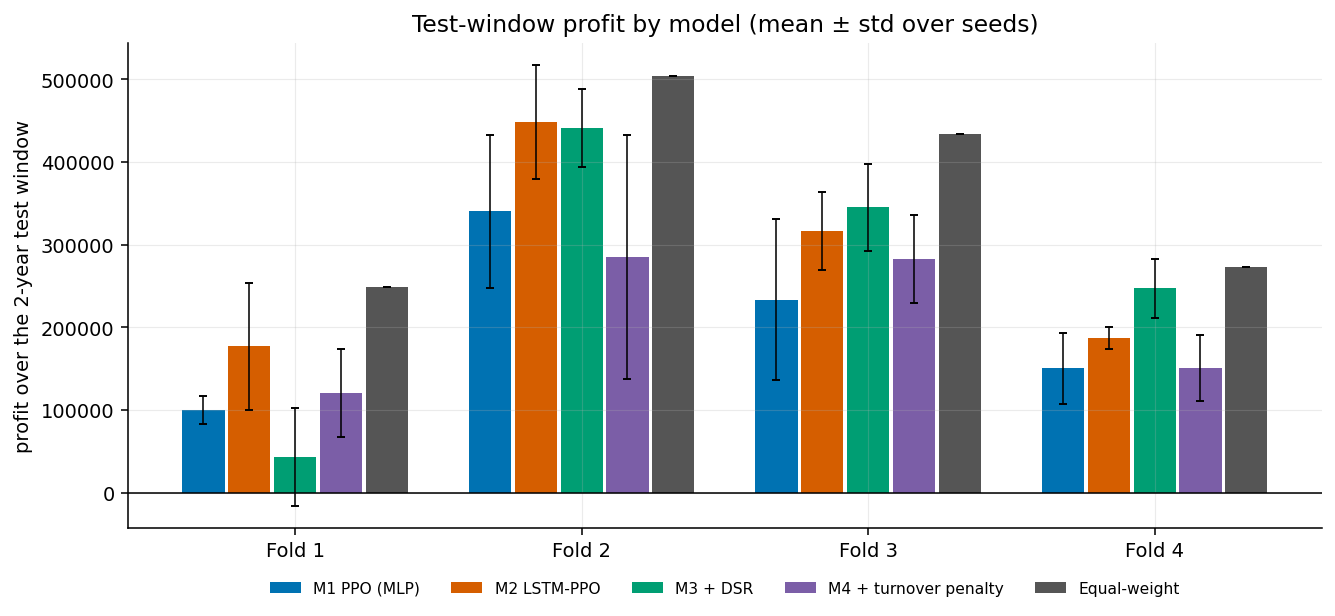
\includegraphics[width=\textwidth]{profit_bars.png}
\caption{Profit per 2-year test window by model.}
\label{fig:profit_bars}
\end{minipage}\hfill
\begin{minipage}{0.49\textwidth}
\centering
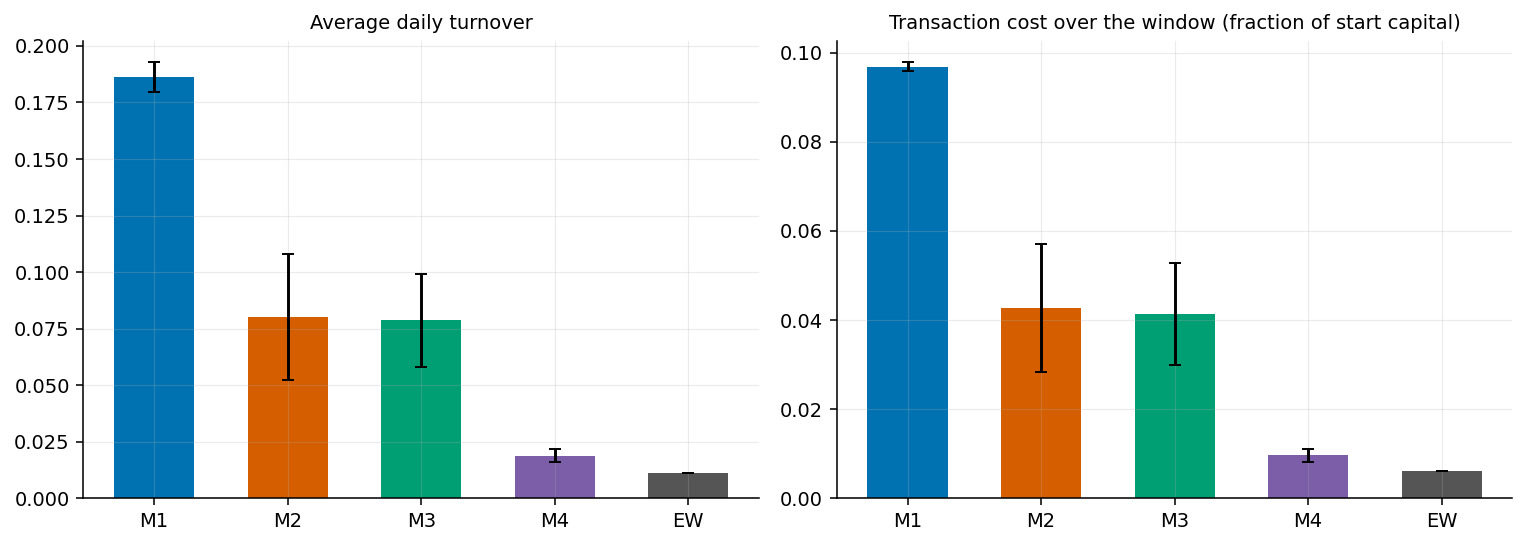
\includegraphics[width=\textwidth]{turnover_cost.png}
\caption{Average daily turnover and transaction costs.}
\label{fig:turnover_cost}
\end{minipage}
\end{figure}

\section{Fold-by-Fold Performance Dynamics}
Table~\ref{tab:per_fold_results} provides the breakdown of cumulative returns across each fold. Performance exhibits marked regime dependence:
\begin{itemize}
    \item \textbf{Fold 1 (2018--2019):} Moderate growth environment. All RL models generate positive return ($10.0\%$ to $17.8\%$), though trailing EW ($24.9\%$).
    \item \textbf{Fold 2 (2020--2021):} Highly volatile pandemic crash and subsequent massive recovery. M2 and M3 capture dramatic gains ($44.8\%$ and $44.1\%$), whereas M4 lagged ($28.5\%$) because its turnover penalty discouraged rapid capital reallocation during the rapid post-crash rebound.
    \item \textbf{Fold 3 (2022--2023):} Inflationary cycle and sector rotation. M3 achieves its strongest risk-adjusted performance with a Sharpe ratio of $1.328$, closely tracking EW ($34.5\%$ vs.\ $43.4\%$).
    \item \textbf{Fold 4 (2024--2025):} Secular bull market. M3 delivers $24.7\%$ return, outperforming M1 and M4.
\end{itemize}

\begin{table}[htbp]
\centering
\small
\caption{Out-of-sample cumulative return (\%) per walk-forward fold (mean $\pm$ standard deviation over seeds).}
\label{tab:per_fold_results}
\begin{tabular}{lccccc}
\toprule
\textbf{Fold Window} & \textbf{Model M1} & \textbf{Model M2} & \textbf{Model M3} & \textbf{Model M4} & \textbf{Equal-Weight} \\
\midrule
Fold 1 (2018--2019) & $10.0 \pm 1.7$ & $17.8 \pm 7.7$ & $4.4 \pm 5.9$ & $12.1 \pm 5.3$ & $\mathbf{24.9}$ \\
Fold 2 (2020--2021) & $34.0 \pm 9.2$ & $44.8 \pm 6.9$ & $44.1 \pm 4.7$ & $28.5 \pm 14.8$ & $\mathbf{50.4}$ \\
Fold 3 (2022--2023) & $23.4 \pm 9.7$ & $31.6 \pm 4.7$ & $34.5 \pm 5.2$ & $28.3 \pm 5.3$ & $\mathbf{43.4}$ \\
Fold 4 (2024--2025) & $15.0 \pm 4.2$ & $18.7 \pm 1.3$ & $24.7 \pm 3.6$ & $15.1 \pm 4.0$ & $\mathbf{27.3}$ \\
\midrule
\textbf{Pooled Mean} & $20.6 \pm 5.1$ & $28.2 \pm 2.0$ & $26.9 \pm 3.3$ & $21.0 \pm 4.2$ & $\mathbf{36.5}$ \\
\bottomrule
\end{tabular}
\end{table}

\section{Equal-Weight Benchmark Outperformance and Gap Decomposition}
In the final experimental test, the passive Equal-Weight benchmark achieved the highest cumulative profit ($36.48\%$ pooled return, Sharpe 1.131), outperforming all four RL models. Rather than obscuring this finding, we perform a rigorous return gap decomposition to understand why active RL underperformed 1/N.

Table~\ref{tab:gap_decomp} decomposes the cumulative return shortfall into two orthogonal components:
\begin{enumerate}
    \item \textbf{Cash Drag:} The return forfeited by holding an uninvested cash allocation during an overall upward-trending market.
    \item \textbf{Stock Choice and Timing:} The differential return resulting from active equity weight deviations relative to equal-weighting across the ten equities.
\end{enumerate}

\begin{table}[htbp]
\centering
\footnotesize
\setlength{\tabcolsep}{4pt}
\caption{Decomposition of cumulative out-of-sample return gap against Equal-Weight (\% points).}
\label{tab:gap_decomp}
\begin{tabular}{lccccc}
\toprule
\textbf{Model} & \textbf{EW Return} & \textbf{Cash Drag} & \textbf{EW Same Cash} & \textbf{Stock Selection} & \textbf{Model Return} \\
\midrule
\textbf{M1 (MLP)} & $135.66$ & $-13.67$ & $121.99$ & $-2.11$ & $119.88$ \\
\textbf{M2 (LSTM)} & $135.66$ & $-9.99$ & $125.67$ & $-2.14$ & $123.53$ \\
\textbf{M3 (+ DSR)} & $135.66$ & $-15.14$ & $120.52$ & $-3.32$ & $117.20$ \\
\textbf{M4 (+ Turn. Pen.)} & $135.66$ & $\mathbf{-42.35}$ & $93.31$ & $-7.84$ & $\mathbf{85.47}$ \\
\bottomrule
\end{tabular}
\end{table}

Table~\ref{tab:avg_weights} reports the average portfolio allocations across the entire evaluation horizon. 

\begin{table}[htbp]
\centering
\scriptsize
\setlength{\tabcolsep}{2.5pt}
\caption{Average asset allocations across models over the out-of-sample evaluation period.}
\label{tab:avg_weights}
\begin{tabular}{lccccccccccc}
\toprule
\textbf{Model} & \textbf{RELI} & \textbf{TCS} & \textbf{HDFCB} & \textbf{ICICIB} & \textbf{ITC} & \textbf{HIND} & \textbf{LT} & \textbf{SUNP} & \textbf{MARU} & \textbf{BHAR} & \textbf{Cash} \\
\midrule
\textbf{M1} & 0.088 & 0.120 & 0.085 & 0.087 & 0.084 & 0.077 & 0.091 & 0.087 & 0.087 & 0.094 & \textbf{0.101} \\
\textbf{M2} & 0.098 & 0.144 & 0.073 & 0.091 & 0.081 & 0.087 & 0.082 & 0.090 & 0.098 & 0.071 & \textbf{0.087} \\
\textbf{M3} & 0.089 & 0.119 & 0.073 & 0.077 & 0.072 & 0.079 & 0.073 & 0.094 & 0.107 & 0.086 & \textbf{0.131} \\
\textbf{M4} & 0.066 & 0.103 & 0.079 & 0.061 & 0.049 & 0.066 & 0.057 & 0.071 & 0.092 & 0.032 & \textbf{0.324} \\
\textbf{EW} & 0.100 & 0.100 & 0.100 & 0.100 & 0.100 & 0.100 & 0.100 & 0.100 & 0.100 & 0.100 & \textbf{0.000} \\
\bottomrule
\end{tabular}
\end{table}

The empirical cause of benchmark outperformance is unequivocal:
\begin{itemize}
    \item Between 2018 and 2025, the Indian equity market experienced a sustained structural bull market. The passive 1/N benchmark remained 100\% invested across all ten large-cap stocks at all times, incurring minimal rebalancing friction ($0.61\%$).
    \item Model M4 learned to allocate an average of \textbf{32.4\%} of its portfolio to cash to minimize volatility and avoid turnover penalties. This cash buffer caused a massive $-42.35\%$ cash drag relative to Equal-Weight. In contrast, stock timing accounted for only $-7.84\%$ deficit.
    \item Thus, M4's lower return was not caused by poor stock picking, but by its risk-averse preference for capital preservation in cash during a high-momentum bull market.
\end{itemize}

\section{M4 Hyperparameter Tuning and Validation Dynamics}
Figure~\ref{fig:m4_sweep} depicts the hyperparameter sweep over $\lambda_{\text{turn}} \in \{0.01, 0.03, 0.1, 0.3\}$ on Fold 1 validation across two random seeds (seeds 0 and 1).

\begin{figure}[htbp]
\centering
\begin{minipage}{0.49\textwidth}
\centering
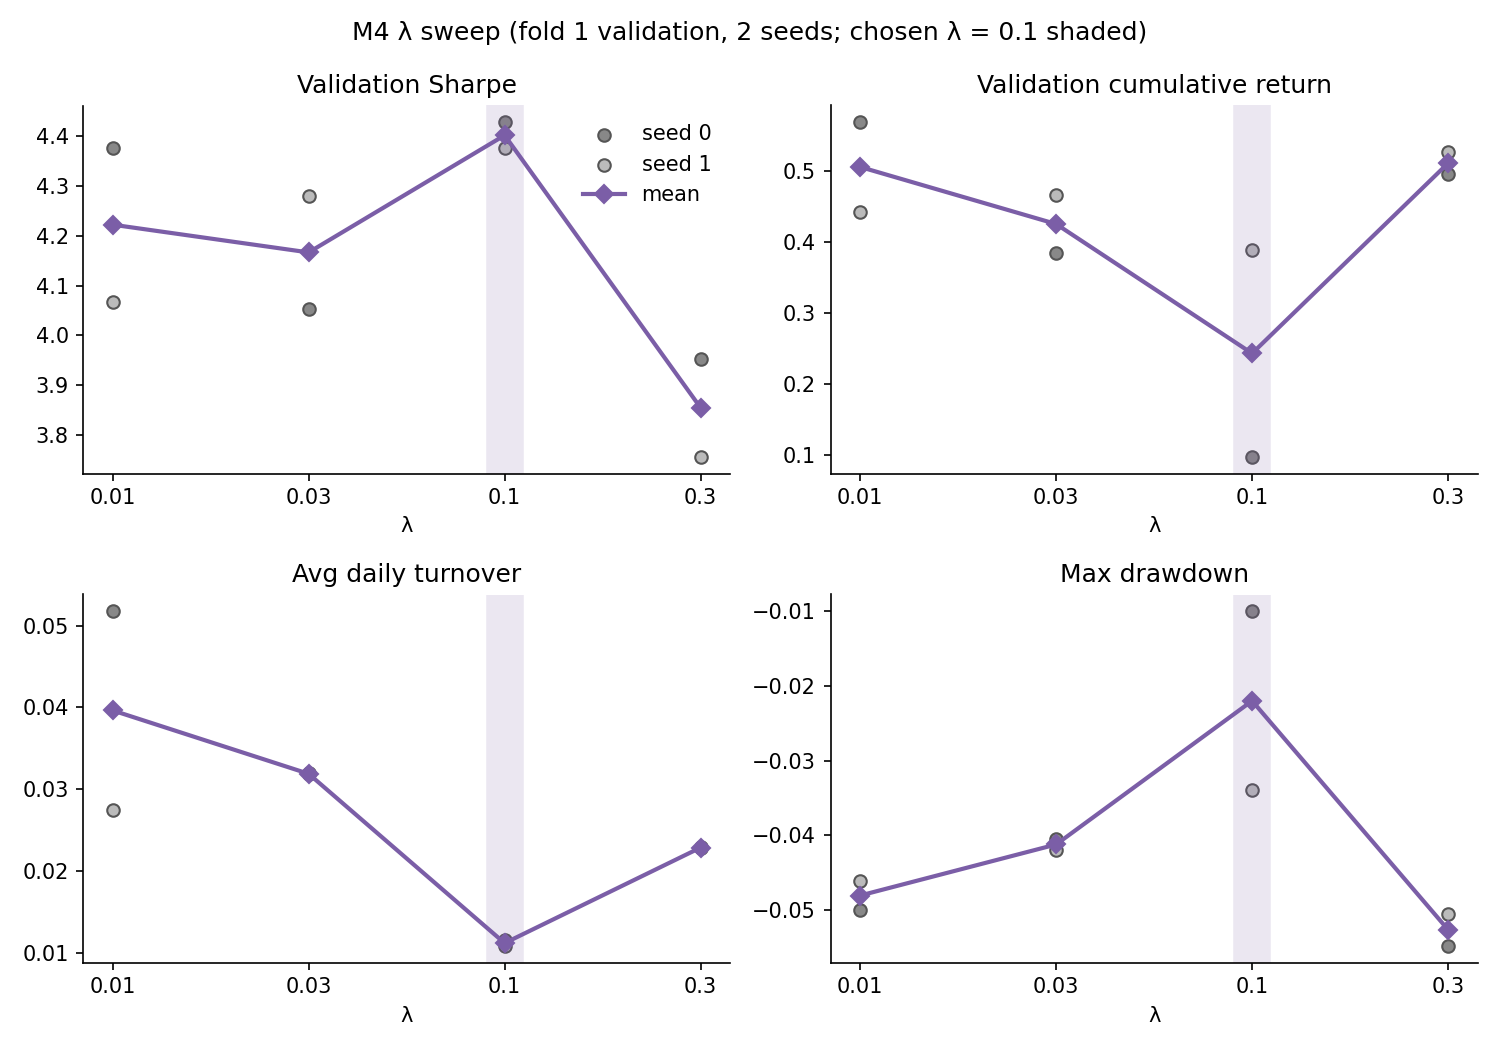
\includegraphics[width=\textwidth]{m4_lambda_sweep.png}
\caption{M4 turnover penalty parameter sweep (chosen $\lambda=0.1$ shaded).}
\label{fig:m4_sweep}
\end{minipage}\hfill
\begin{minipage}{0.49\textwidth}
\centering
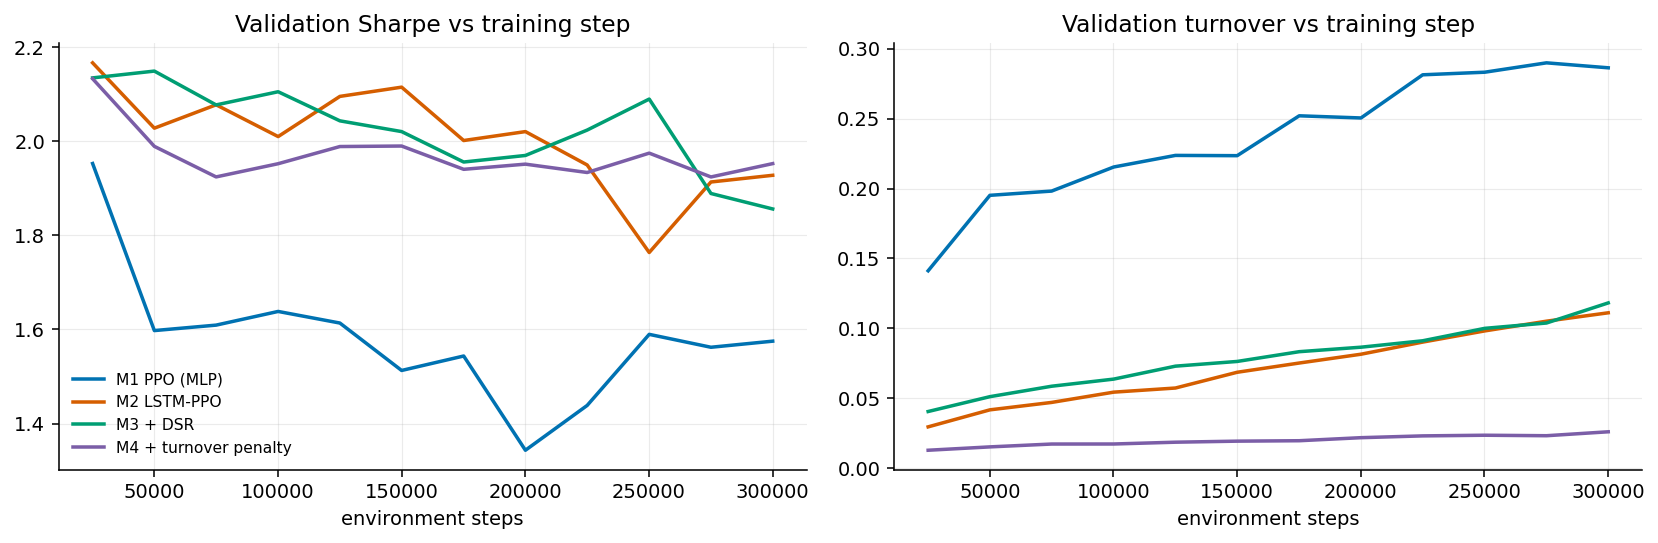
\includegraphics[width=\textwidth]{validation_curves.png}
\caption{Validation Sharpe and turnover dynamics over 300,000 steps.}
\label{fig:val_curves}
\end{minipage}
\end{figure}

The grid sweep demonstrates that $\lambda = 0.1$ achieved the optimal trade-off on Fold 1 validation, maximizing the mean validation Sharpe ratio ($4.40$) while curtailing validation drawdown to $-2.2\%$. At $\lambda = 0.01$, turnover remains high ($0.040$), whereas at $\lambda = 0.3$, the penalty stifles necessary reallocations. We explicitly note as a limitation that $\lambda_{\text{turn}} = 0.1$ was selected on Fold 1 alone across two seeds and applied frozen across all folds. Finally, the validation curves show clear over-training beyond 100,000 steps, highlighting the critical importance of checkpoint early stopping.

\chapter{Limitations and Future Work}
\label{ch:limitations}

\section{Methodological and Empirical Limitations}
While this project provides a rigorous, controlled investigation into reinforcement learning for portfolio management, several realistic limitations must be acknowledged:

\subsection{Passive Benchmark Outperformance and Survivorship Bias}
The equal-weight 1/N strategy demonstrated superior cumulative profit and Sharpe ratio compared to all deep RL agents. This is attributable to two primary factors:
\begin{enumerate}
    \item \textbf{Survivorship Bias in Equity Selection:} The 10 stocks selected (e.g., Reliance, TCS, HDFC Bank, ICICI Bank) represent established corporate leaders that survived and prospered over the 2011--2025 window. In an asset universe characterised by strong upward drift, a passive, fully-invested allocation captures market beta at negligible transaction costs ($0.61\%$).
    \item \textbf{Cash Drag from Learned Risk Aversion:} The continuous Dirichlet policy learned to maintain cash buffers (up to $32.4\%$ in M4) to guard against volatility. While this successfully curbed maximum drawdown to $-16.04\%$, it penalized nominal capital compounding during bull markets.
\end{enumerate}

\subsection{Market Regime Dependence and Single-Epoch Hyperparameter Selection}
As disclosed in Chapter~\ref{ch:results}, the turnover regularisation coefficient $\lambda_{\text{turn}} = 0.1$ was tuned strictly on Fold 1 validation across two seeds. Subsequent folds encompassed vastly different market regimes—notably the COVID-19 crash of March 2020 (Fold 2) and the global inflationary cycle of 2022 (Fold 3). A constant hyperparameter tuned in a calm market proved overly restrictive during volatile recovery phases where rapid rebalancing was necessary.

\subsection{Simplified Execution and Market Impact Assumptions}
The environment models execution costs as a fixed proportional fee $c_{\text{trans}} = 0.001$ ($10\text{ bps}$). While appropriate for retail and liquid institutional execution, this model neglects:
\begin{itemize}
    \item Non-linear market impact and price slippage for large order sizes.
    \item Intraday execution dynamics (trades are executed at the official daily closing price).
    \item Short-selling constraints and margin financing costs.
\end{itemize}

\subsection{Computational and Stochastic Architecture Constraints}
Due to computational constraints, policies were restricted to a single-layer LSTM with 512 hidden units, trained for 300,000 steps per run. Furthermore, continuous Dirichlet sampling exhibits inherent stochasticity, leading to noticeable variance across random seeds (e.g., Fold 2 return std $\pm 14.8\%$ in M4).

\section{Directions for Future Research}
The insights gained from this study motivate several promising avenues for future inquiry:
\begin{enumerate}
    \item \textbf{Dynamic and Adaptive Turnover Regularisation:} Rather than maintaining a static penalty $\lambda_{\text{turn}}$, future models could employ adaptive penalty scheduling conditioned on real-time market volatility (e.g., VIX) or learned meta-policy networks.
    \item \textbf{Attention and Transformer Backbones:} Replacing recurrent LSTM cells with temporal multi-head attention mechanisms (such as Temporal Fusion Transformers) could enhance the extraction of long-range cross-asset correlations.
    \item \textbf{Macroeconomic and Alternative Feature Integration:} Augmenting technical indicators with macroeconomic variables (interest rates, crude oil prices, USD/INR foreign exchange rates) and sentiment features from financial disclosures.
    \item \textbf{Dynamic Cash Hurdles:} Incorporating an active risk-free interest rate yield on the cash reserve to mitigate the harsh cash drag observed in equity bull markets.
\end{enumerate}

\chapter{Conclusion}
\label{ch:conclusion}

\section{Summary of Research Findings}
This B.Tech.\ project developed, implemented, and empirically evaluated a continuous Actor--Critic Deep Reinforcement Learning framework for daily portfolio allocation across ten major equities on the National Stock Exchange of India. By formulating the policy over a multivariate Dirichlet distribution, the agent generated continuous target allocations that strictly preserved the portfolio simplex manifold. Through an extensive, strictly controlled four-stage ablation study (M1--M4) evaluated across four rolling walk-forward folds and three random seeds (2018--2025), this study isolated the individual contributions of temporal memory, risk-sensitive rewards, and turnover regularisation.

\section{Answers to Research Questions}
We conclude by providing direct, evidence-based answers to the four core research questions:

\begin{itemize}
    \setlength{\itemsep}{3pt}
    \setlength{\parskip}{1pt}
    \item \textbf{RQ1 (Temporal Architecture):} \textit{Does an LSTM-based recurrent encoder improve out-of-sample risk-adjusted returns and policy stability compared to an MLP encoder?}
    
    \textbf{Answer: Yes, unequivocally.} Transitioning from the instantaneous MLP (M1) to the sequence-aware LSTM (M2) improved the out-of-sample Sharpe ratio by $+0.201$ (from $0.714$ to $0.915$, 95\% CI $[+0.156, +0.246]$) with consistent improvements across all four folds ($4/4$). Moreover, the LSTM reduced daily turnover from $0.186$ to $0.080$ and cut total transaction costs by more than half (from $9.68\%$ to $4.27\%$), demonstrating that temporal memory is essential for filtering market noise and preventing counterproductive daily portfolio churning.

    \item \textbf{RQ2 (Risk-Adjusted Reward):} \textit{Does transitioning from raw net return to the Differential Sharpe Ratio (DSR) lead to improved Sharpe ratios and reduced drawdowns?}
    
    \textbf{Answer: Partially, with nuanced trade-offs.} The DSR reward (M3) yielded an incremental Sharpe delta of $+0.003$ ($[-0.295, +0.222]$) relative to M2. While DSR demonstrated strong performance in later regimes (Sharpe $1.328$ in Fold 3 and $1.164$ in Fold 4), its online variance estimation slightly depressed cumulative profit during aggressive bull markets ($26.93\%$ vs.\ $28.23\%$).

    \item \textbf{RQ3 (Turnover Regularisation):} \textit{Does augmenting the reward with an explicit quadratic turnover penalty effectively suppress portfolio turnover and transaction costs without destroying wealth accumulation?}
    
    \textbf{Answer: Yes, decisively.} Incorporating the quadratic turnover penalty in Model M4 suppressed average daily turnover from $0.079$ to $0.019$ ($[-0.082, -0.044]$, improved in $12/12$ pairs), reducing transaction costs to just $0.97\%$ of starting capital. Crucially, M4 delivered the shallowest maximum drawdown of any evaluated model ($-16.04\%$, an improvement of $+3.90\%$ over M3), successfully demonstrating that explicit turnover regularisation stabilizes portfolio execution under proportional transaction costs.

    \item \textbf{RQ4 (Benchmark Competitiveness):} \textit{Can a model-free continuous actor-critic agent outperform a passively rebalanced equal-weight benchmark in a high-friction Indian equity universe?}
    
    \textbf{Answer: No.} The passive Equal-Weight benchmark achieved superior cumulative return ($36.48\%$) and Sharpe ratio ($1.131$). Our gap decomposition revealed that this underperformance was predominantly driven by \textit{cash drag} ($-42.35\%$ in M4) caused by the policy's learned risk-averse allocation to cash ($32.4\%$) during an extended secular bull market. In asset universes characterised by strong macroeconomic upward drift, overcoming the beta advantage and negligible cost ($0.61\%$) of passive 1/N diversification remains an formidable challenge for active reinforcement learning agents.
\end{itemize}

\section{Concluding Remarks}
In summary, this research demonstrates that deep reinforcement learning can autonomously discover disciplined risk-management and cost-conscious trading policies in real financial markets. While active outperformance against passive broad-market equities is bounded by cash drag and execution costs, the controlled ablation methodology established in this thesis provides a rigorous scientific template for future investigations in quantitative financial machine learning.


%% ===== BIBLIOGRAPHY =====
\newpage
\bibliographystyle{plainnat}
\bibliography{references}

\end{document}
